\documentclass[xcolor=dvipsnames]{beamer}

\usepackage{graphicx}
\usepackage{listings}
\usepackage{comment}
\usepackage{float}
\usepackage{array}
\usepackage{tikz}
\usepackage{textcomp}
\usepackage{multicol}
\usepackage{grffile}
%\usepackage[dvips]{graphics}

\usetikzlibrary{arrows}

\usetheme{Frankfurt}
%\usecolortheme[named=OliveGreen]{structure}
%\usefonttheme{serif}
\setbeamertemplate{navigation symbols}{}
\setbeamertemplate{frametitle}[default][center]

\newcommand{\ReadArrowType}{latex}

\newcommand{\BidirectedEdgeForward}[2]{
        \tikz[>=triangle 45,baseline]
        \draw[>->,thin] (0,0.1) node[anchor=east] {#1} --
                        (0.8,0.1) node[anchor=west] {#2};}

\newcommand{\LengthVar}{L}

\begin{document}
\title{A Bidirected String Graph Model of Genome Assembly}
\author{Eric Biggers}
\institute{Macalester College}
\date{April 16, 2014}
%\titlegraphic{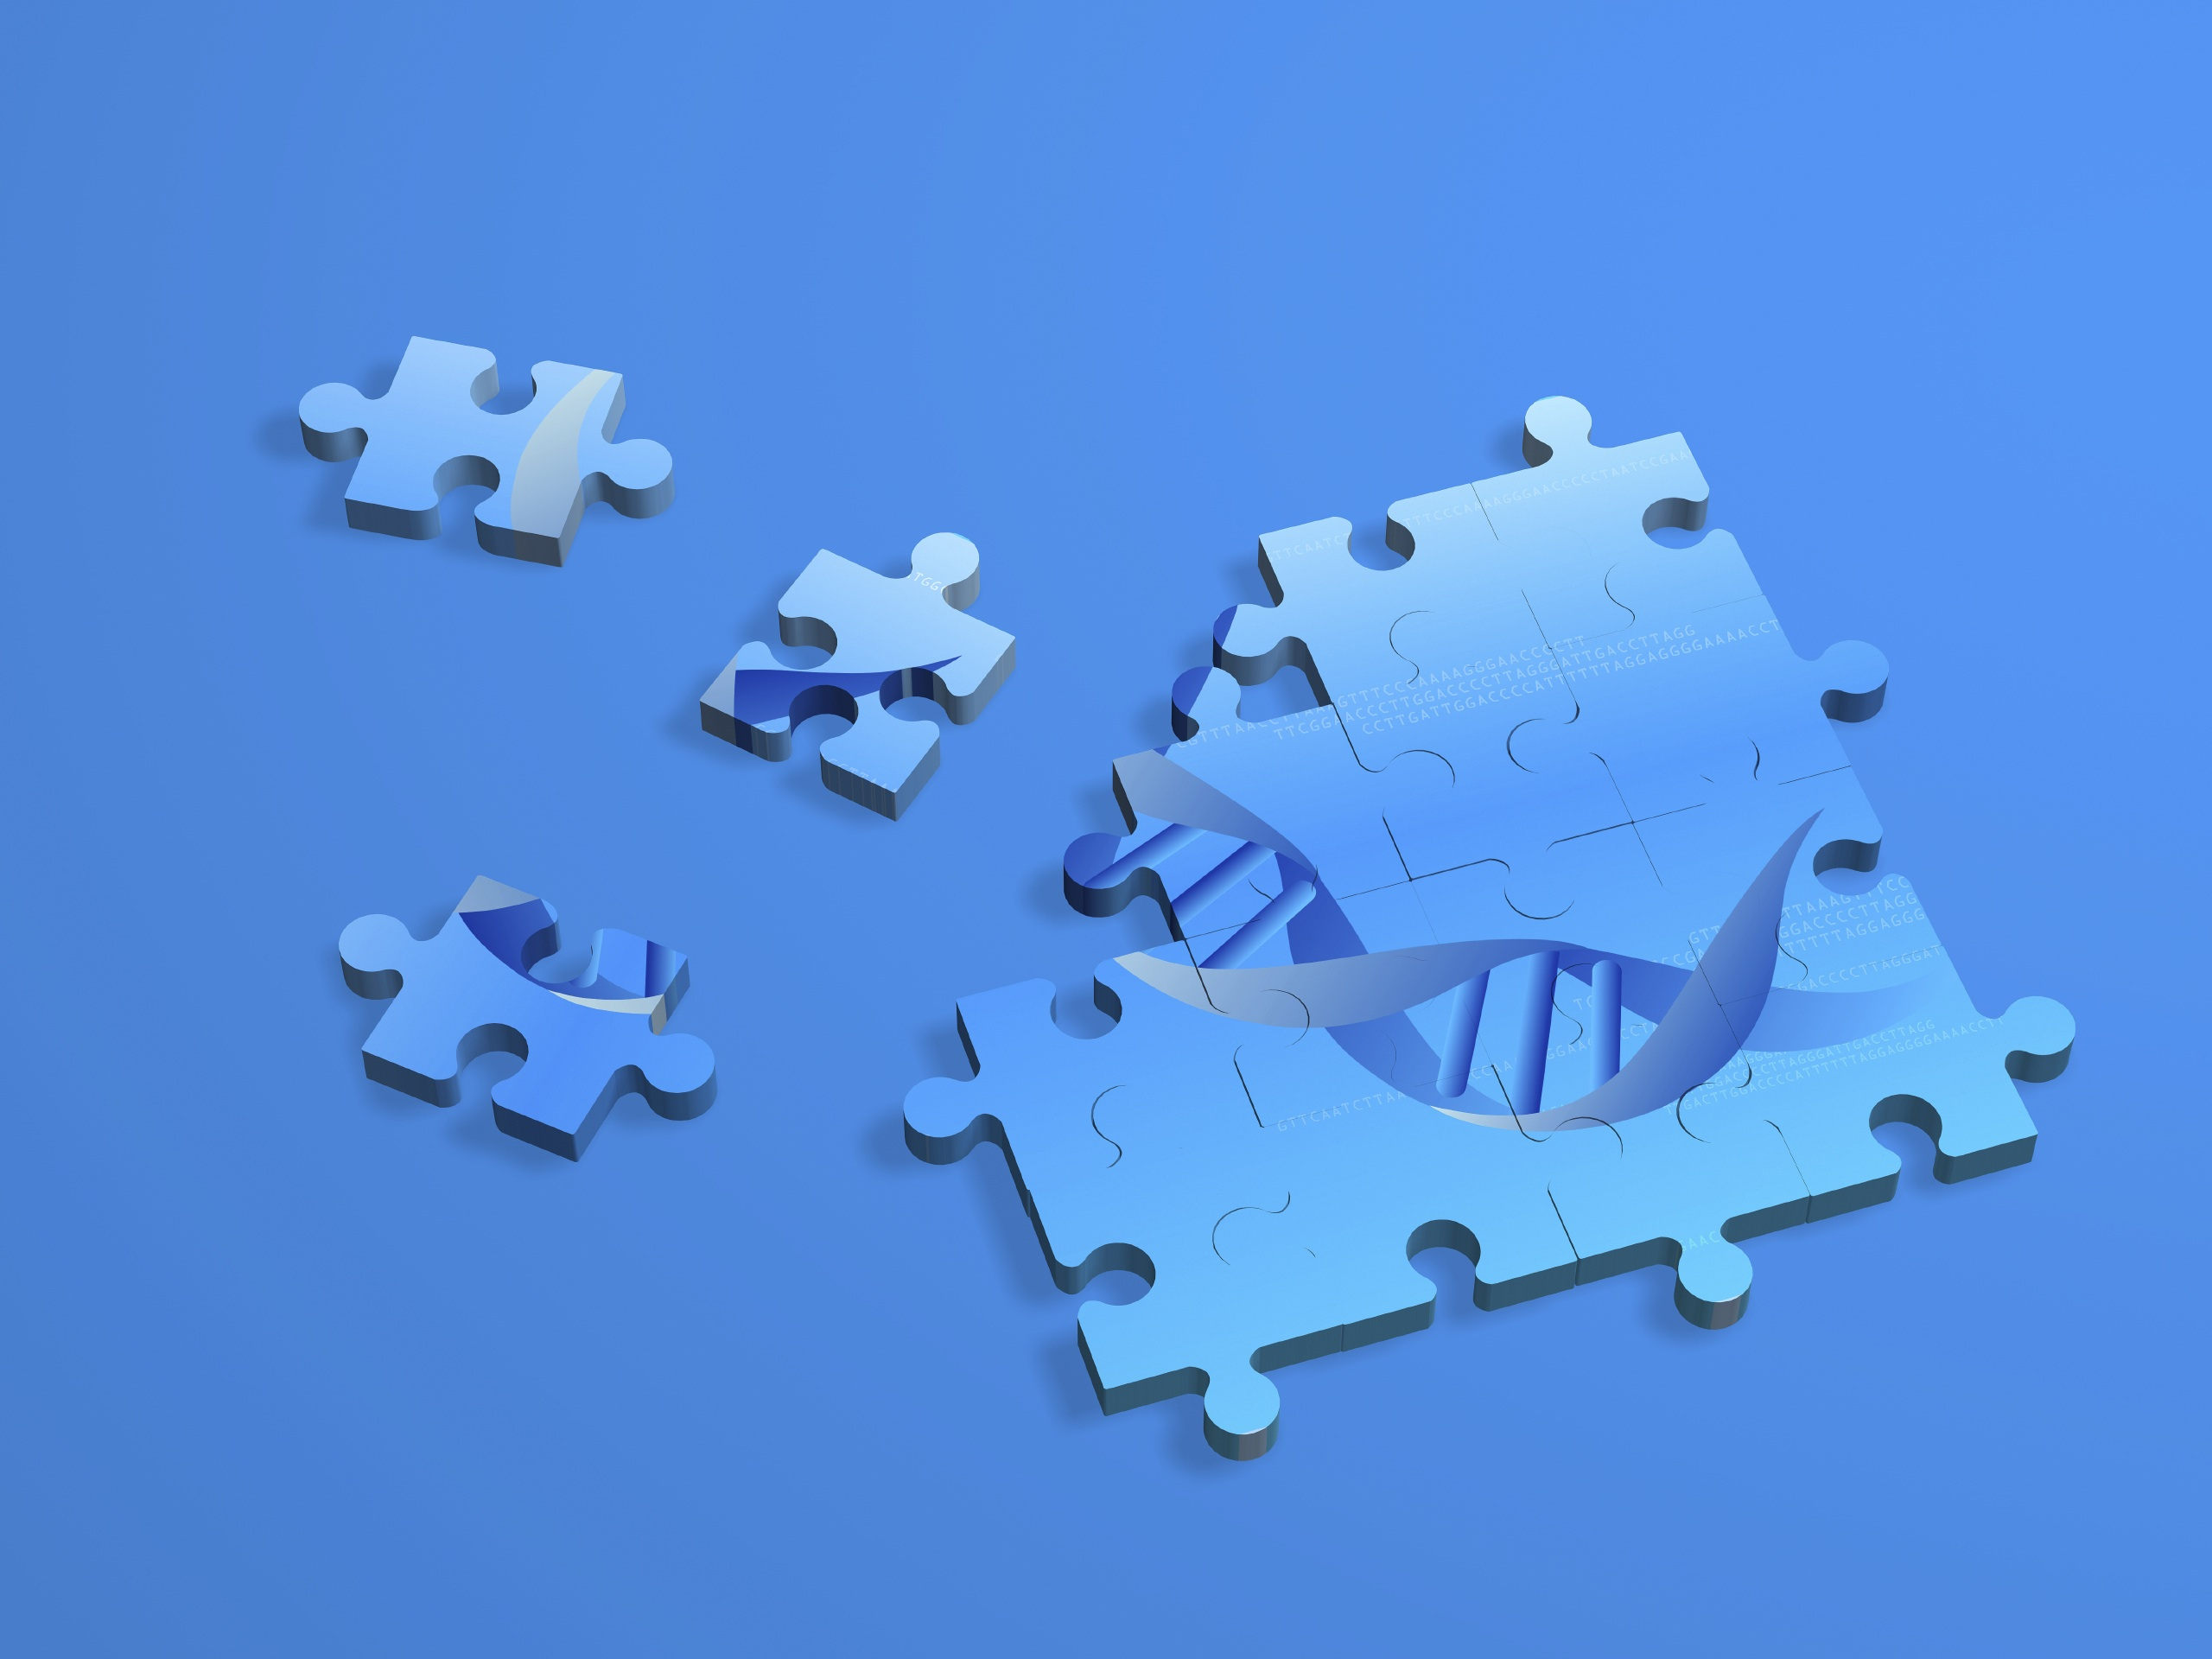
\includegraphics[width=\textwidth,clip=true,trim=0 300 0 500]{puzzle.jpg}}


\definecolor{darkyellow}{rgb}{0.65,0.60,0.00}
\definecolor{darkgreen}{rgb}{0.00,0.40,0.00}
\newcommand\A{\textcolor{darkyellow}{A}}
\newcommand\T{\textcolor{darkgreen}{T}}
\newcommand\G{\textcolor{red}{G}}
\newcommand\C{\textcolor{blue}{C}}

\frame{\titlepage}

\begin{frame}{Outline}
    \vspace{1cm}
    \begin{enumerate}
        \item Introduction to genome sequencing \& assembly
        \item Modeling genome assembly using bidirected string graphs
    \end{enumerate}
    %\begin{minipage}{0.49\textwidth}
        %\begin{center}
            %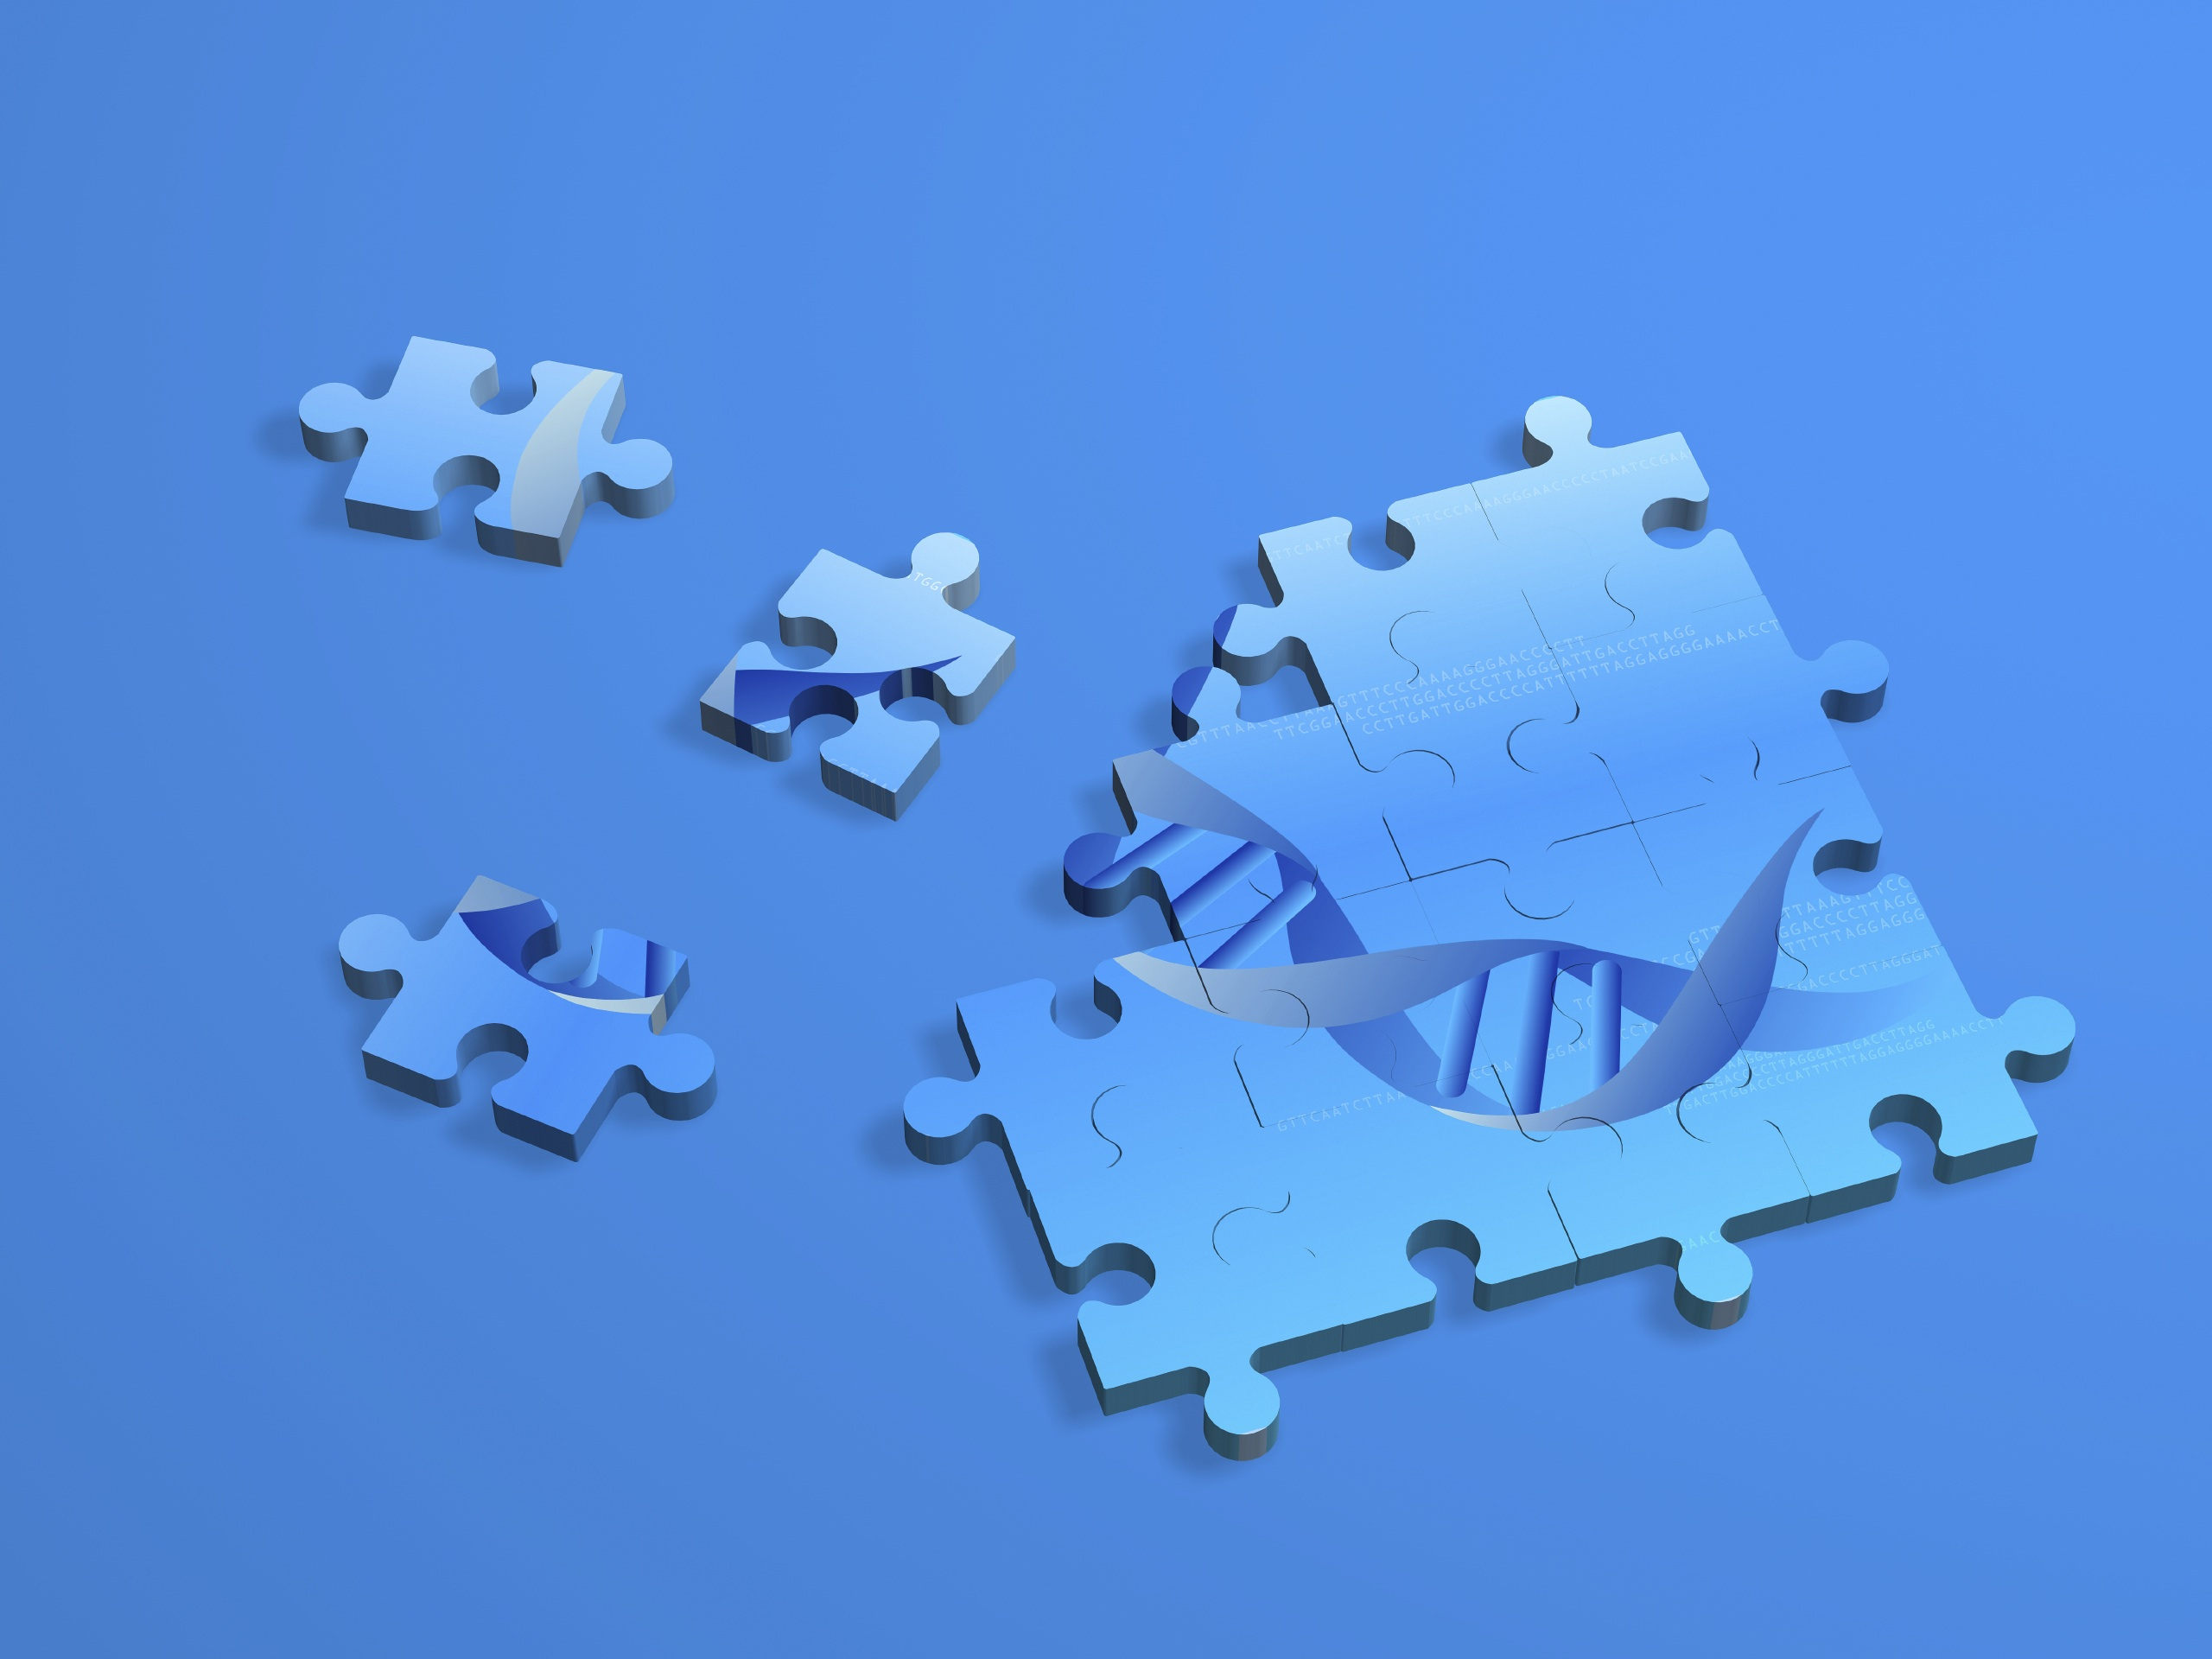
\includegraphics[width=\textwidth]{puzzle.jpg}
        %\end{center}
    %\end{minipage}
    %\begin{minipage}{0.49\textwidth}
    \begin{center}
        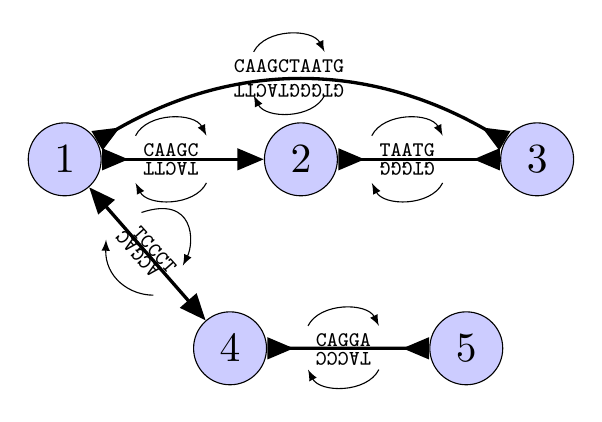
\begin{tikzpicture}[>=triangle 45,scale=1.5,every node/.style={scale=1.5}]
            \node[circle,fill=blue!20,draw=black] (1) at (+0.0, +0.0) {1};
            \node[circle,fill=blue!20,draw=black] (2) at (+2.0, +0.0) {2};
            \node[circle,fill=blue!20,draw=black] (3) at (+4.0, +0.0) {3};
            \node[circle,fill=blue!20,draw=black] (4) at (+1.4, -1.6) {4};
            \node[circle,fill=blue!20,draw=black] (5) at (+3.4, -1.6) {5};
            \draw[>->,style=very thick] (1) edge (2);
            \draw[>-<,style=very thick] (2) edge (3);
            \draw[>-<,style=very thick,bend left] (1) edge (3);
            \draw[<->,style=very thick] (1) edge (4);
            \draw[>-<,style=very thick] (4) edge (5);

            %%%%%%%%%%%%%%%%%%%%%%%%%%%%%%%%%%%
            % 1E -> 2E
            \draw (0.9, -0.1) node[anchor=south] { \rotatebox{0}{\tiny \tt CAAGC}};
            \draw[->,style=thin,>=latex]
                (0.6, 0.2) ..  controls (0.7, 0.4) and (1.1, 0.4) ..  (1.2, 0.2);

            % 2B -> 1B
            \draw (0.9, 0.1) node[anchor=north] { \rotatebox{180}{\tiny \tt TACTT}};
            \draw[<-,style=thin,>=latex]
                (0.6, -0.2) ..  controls (0.7, -0.4) and (1.1, -0.4) ..  (1.2, -0.2);
            %%%%%%%%%%%%%%%%%%%%%%%%%%%%%%%%%%%


            %%%%%%%%%%%%%%%%%%%%%%%%%%%%%%%%%%%
            % 2E -> 3B
            \draw (2.9, -0.1) node[anchor=south] { \rotatebox{0}{\tiny \tt TAATG}};
            \draw[->,style=thin,>=latex]
                (2.6, 0.2) ..  controls (2.7, 0.4) and (3.1, 0.4) ..  (3.2, 0.2);

            % 3E -> 2B
            \draw (2.9, 0.1) node[anchor=north] { \rotatebox{180}{\tiny \tt GTGGG}};
            \draw[<-,style=thin,>=latex]
                (2.6, -0.2) ..  controls (2.7, -0.4) and (3.1, -0.4) ..  (3.2, -0.2);
            %%%%%%%%%%%%%%%%%%%%%%%%%%%%%%%%%%%

            % 1E -> 3B
            \draw (1.9, 0.61) node[anchor=south] { \rotatebox{0}{\tiny \tt CAAGCTAATG}};
            \draw[->,style=thin,>=latex]
                (1.6, 0.91) ..  controls (1.7, 1.11) and (2.1, 1.11) ..
                (2.2, 0.91);

            % 3E -> 1B
            \draw (1.9, 0.76) node[anchor=north] { \rotatebox{180}{\tiny \tt GTGGGTACTT}};
            \draw[<-,style=thin,>=latex]
                (1.6, 0.54) ..  controls (1.7, 0.34) and (2.1, 0.34) ..
                (2.2, 0.54);
            %%%%%%%%%%%%%%%%%%%%%%%%%%%%%%%%%%%

            % 1B -> 4E
            \draw (0.76, -1.10) node[anchor=south] { \rotatebox{312}{\tiny \tt TCCCT}};
            \draw[->,style=thin,>=latex]
                (0.65, -0.45) ..  controls (1.1, -0.3) and (1.1, -0.7) ..
                (1.0, -0.9);

            % 4B -> 1E
            \draw (0.62, -0.47) node[anchor=north] { \rotatebox{132}{\tiny \tt ACGAC}};
            \draw[<-,style=thin,>=latex]
                (0.35, -0.68) ..  controls (0.34, -1) and (0.55, -1.15) ..
                (0.75, -1.15);
            %%%%%%%%%%%%%%%%%%%%%%%%%%%%%%%%%%%

            % 4E -> 5B
            \draw (2.36, -1.71) node[anchor=south] { \rotatebox{0}{\tiny \tt CAGGA}};
            \draw[->,style=thin,>=latex]
                (2.06, -1.41) ..  controls (2.16, -1.21) and (2.56, -1.21) ..
                (2.66, -1.41);

            % 5E -> 4B
            \draw (2.36, -1.51) node[anchor=north] { \rotatebox{180}{\tiny \tt TACCC}};
            \draw[<-,style=thin,>=latex]
                (2.06, -1.78) ..  controls (2.16, -1.98) and (2.56, -1.98) ..
                (2.66, -1.78);
            %%%%%%%%%%%%%%%%%%%%%%%%%%%%%%%%%%%

        \end{tikzpicture}
        %
        %
        % CATTAGCTTGGTCGTGGGTACTTTCCCTCAGGA
        %
        % >33333333333>
        %      <22222222222<
        %           <11111111111<
        %                >44444444444>
        %                     <55555555555<
    \end{center}
    %\end{minipage}
\end{frame}

\begin{frame}{Genomes}
    \begin{minipage}{0.75\textwidth}
        \begin{itemize}
            \item A {\bf genome} is an organism's genetic material
            \item A genome consists of one or more {\bf DNA molecules}
            \item DNA molecules are double-stranded sequences of paired
                  nucleotides
            \item A pairs with T; C pairs with G
            \item Each paired nucleotide is a {\bf base pair} (abbreviation: {\bf bp})
        \end{itemize}
            \begin{center}
                {\tt {\bf $\leftarrow$}\G{}\T{}\T{}\G{}\C{}\T{}\A{}\T{}\A{}\A{}\A{}\T{}\A{}\C{}\G{}\G{}\G{}\T{}\C{}\A{}\T{}\G{}\G{}\T{}\A{}\T{}\T{}\T{}\A{}\C{}\C{}\G{}{\bf $\leftarrow$}} \\
                \vspace{-0.14cm}
                {\tt                     ||||||||||||||||||||||||||||||||} \\
                \vspace{-0.14cm}
                {\tt {\bf $\rightarrow$}\C{}\A{}\A{}\C{}\G{}\A{}\T{}\A{}\T{}\T{}\T{}\A{}\T{}\G{}\C{}\C{}\C{}\A{}\G{}\T{}\A{}\C{}\C{}\A{}\T{}\A{}\A{}\A{}\T{}\G{}\G{}\C{}{\bf $\rightarrow$}}
            \end{center}
    \end{minipage}
    \begin{minipage}{0.23\textwidth}
        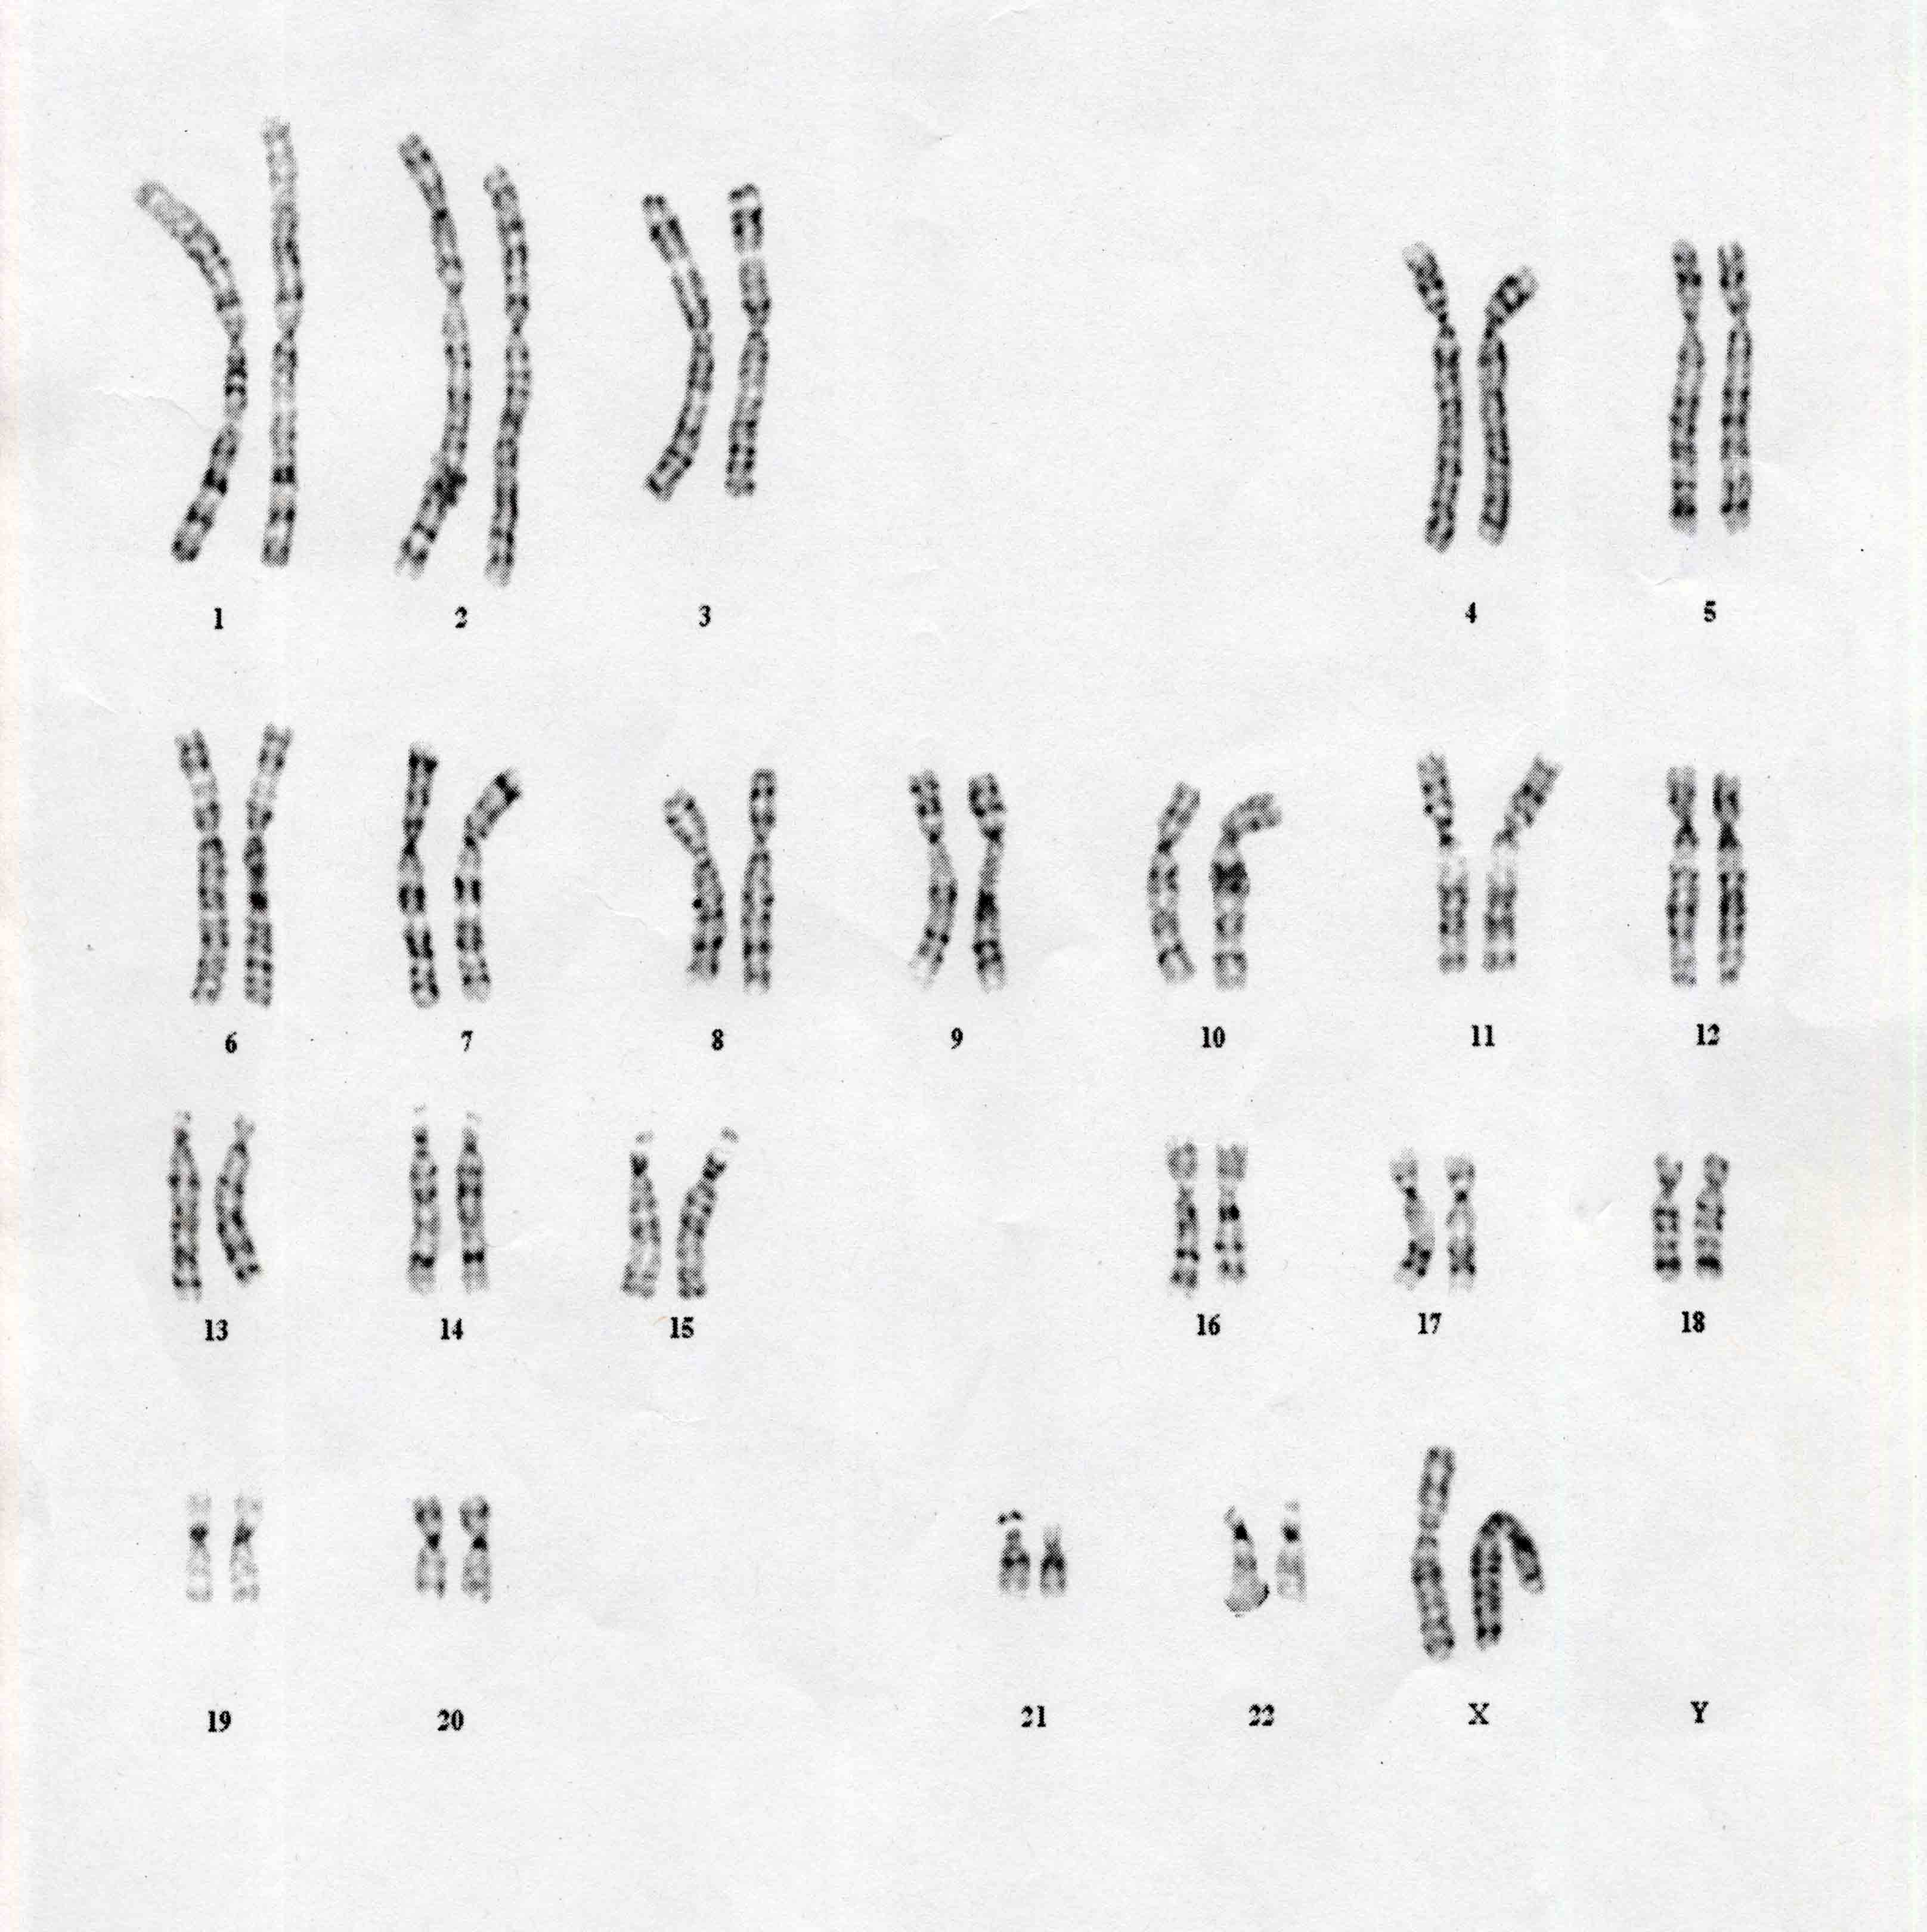
\includegraphics[width=1.0\textwidth]{HumanKaryotype.jpg} \\
        \vspace{0.05cm}
        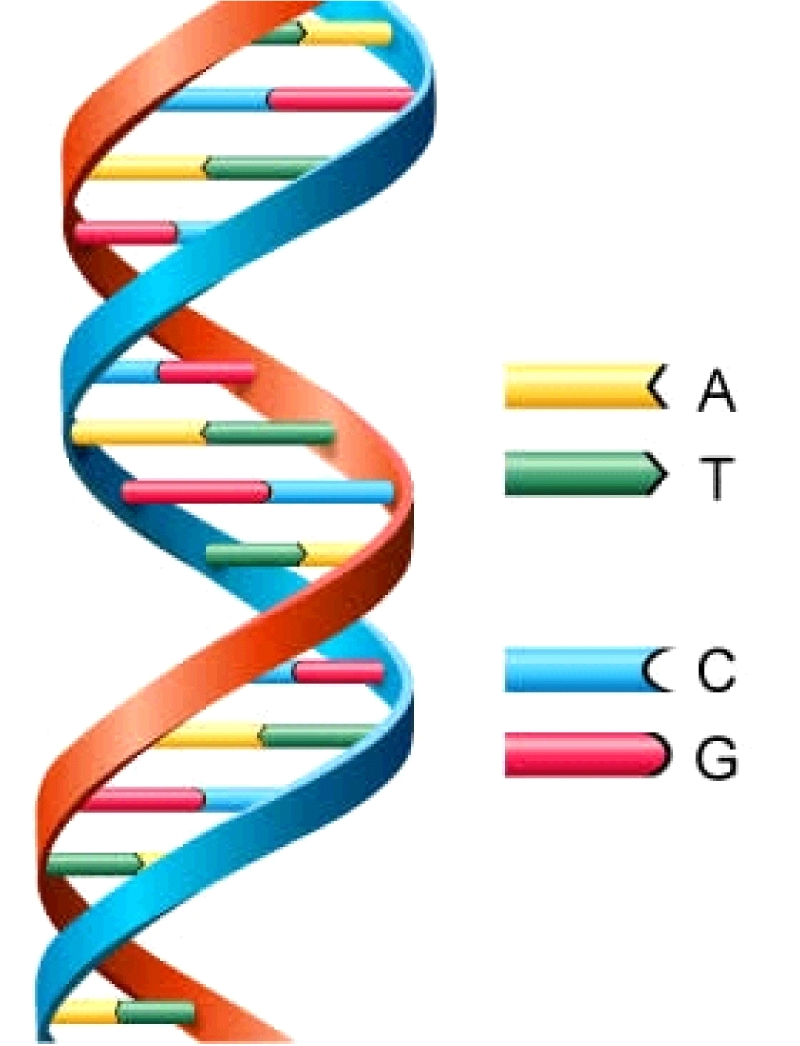
\includegraphics[width=1.0\textwidth]{DNA.jpg}
    \end{minipage}
\end{frame}

\begin{frame}{Genome sizes}
    \begin{tabular}{|m{2.8cm}m{2.6cm}|m{3.8cm}|}
        \hline
        \multicolumn{2}{|c|}{ {\bf Organism }} & {\bf Genome size (appox.)} \\
        \hline
        { \it Escherichia coli}
        &
        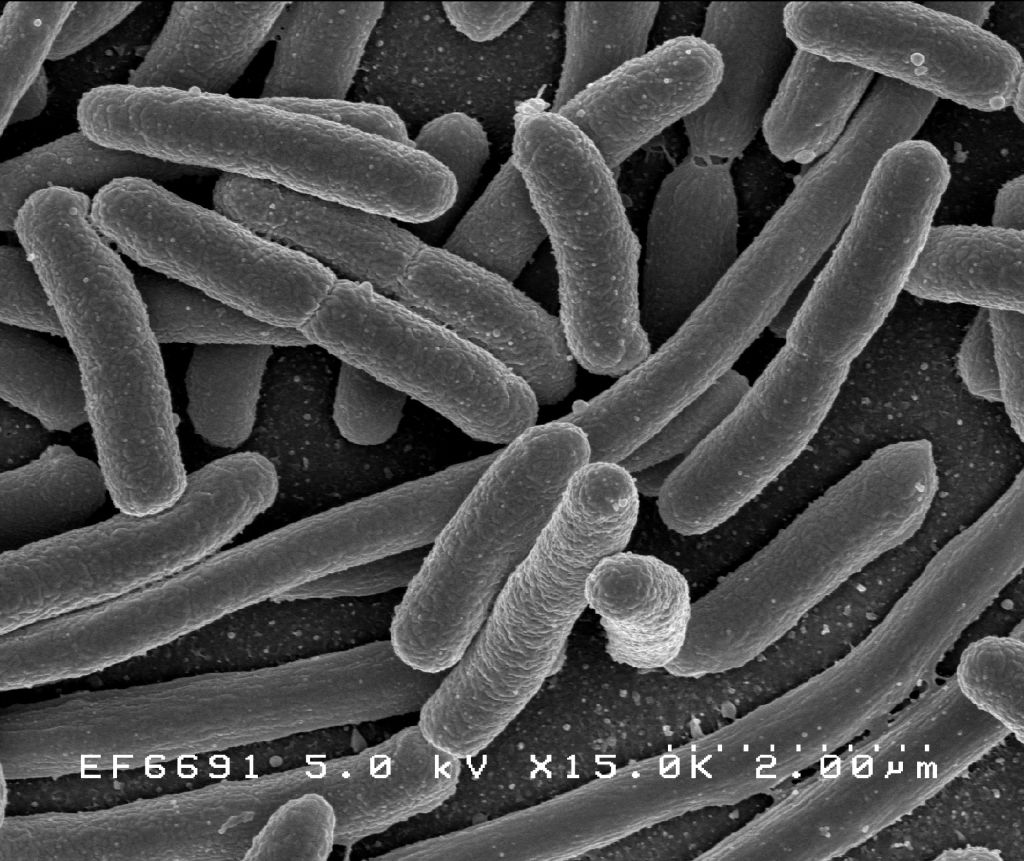
\includegraphics[height=0.15\textwidth]{E_coli.jpg}
        & 4,600,000 bp \\
        \hline
        {\it Ananas comosus} &
        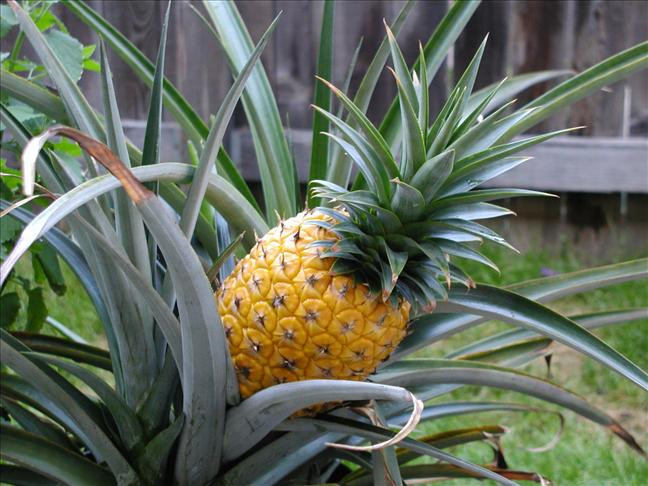
\includegraphics[height=0.15\textwidth]{Pineapple.jpg}
        & 500,000,000 bp \\
        \hline
        {\it Homo sapiens} &
        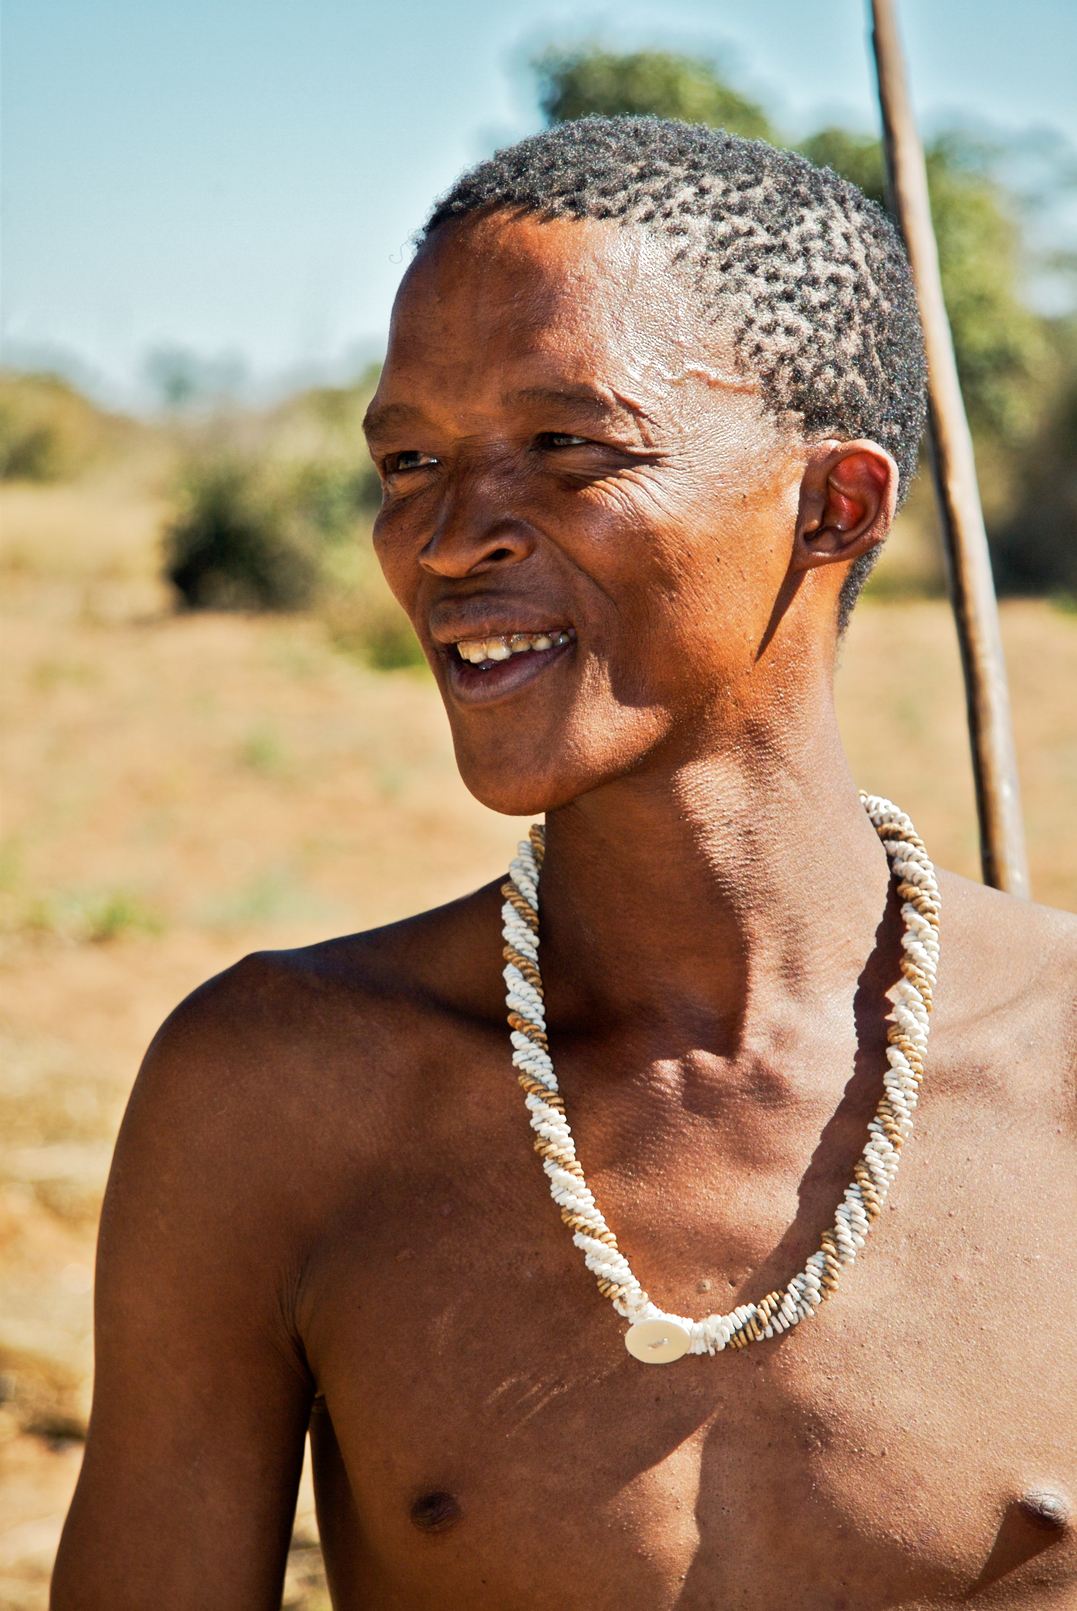
\includegraphics[height=0.15\textwidth,clip=true,trim=0 180 0 0]{Human.jpg}
        & 3,200,000,000 bp \\
        \hline
        {\it Pinus taeda} &
        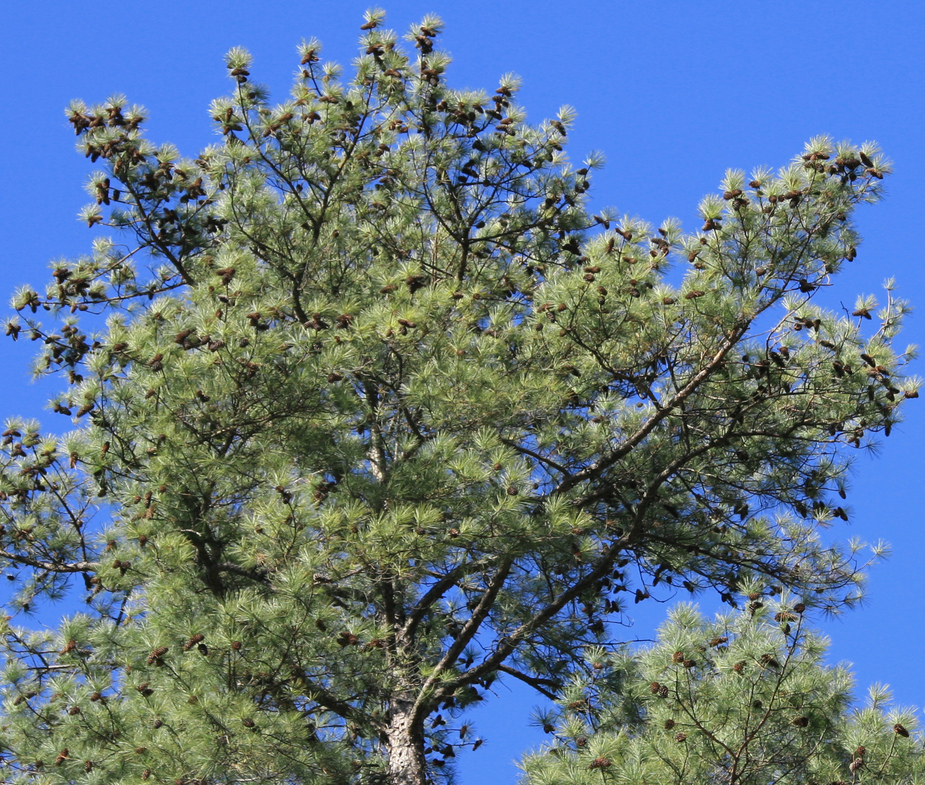
\includegraphics[height=0.15\textwidth]{LoblollyPine.jpg}
        & 23,200,000,000 bp \\
        \hline
    \end{tabular}
\end{frame}

\begin{frame}{De novo whole genome shotgun sequencing}
    \begin{minipage}{0.66\textwidth}
        \begin{itemize}
            \item Currently the fastest and cheapest way to sequence an entire
                  new genome
            \item Relies on one of several technologies, each of which can only
                sequence short pieces of DNA
            \item Step 1: Lab work
                \begin{itemize}
                    \item Obtain a DNA sample
                    \item Break DNA into small fragments
                    \item Sequence the fragments
                \end{itemize}
            \item Step 2: Computational work
                \begin{itemize}
                    \item Given the sequenced fragments, reconstruct the original genome
                \end{itemize}
        \end{itemize}
    \end{minipage}
    \begin{minipage}{0.32\textwidth}
        \begin{center}
            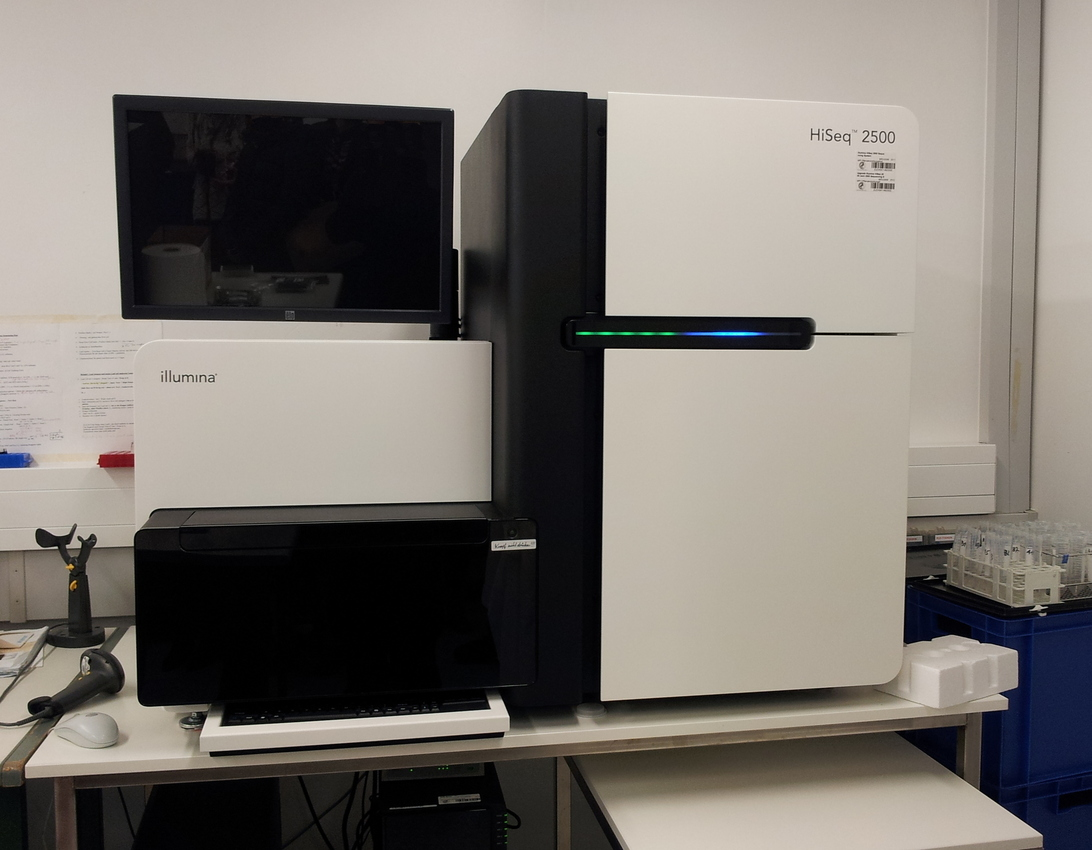
\includegraphics[width=1.0\textwidth]{Illumina_HiSeq_2500.jpg} \\
                Illumina HiSeq 2500 \\
            \vspace{0.2cm}
            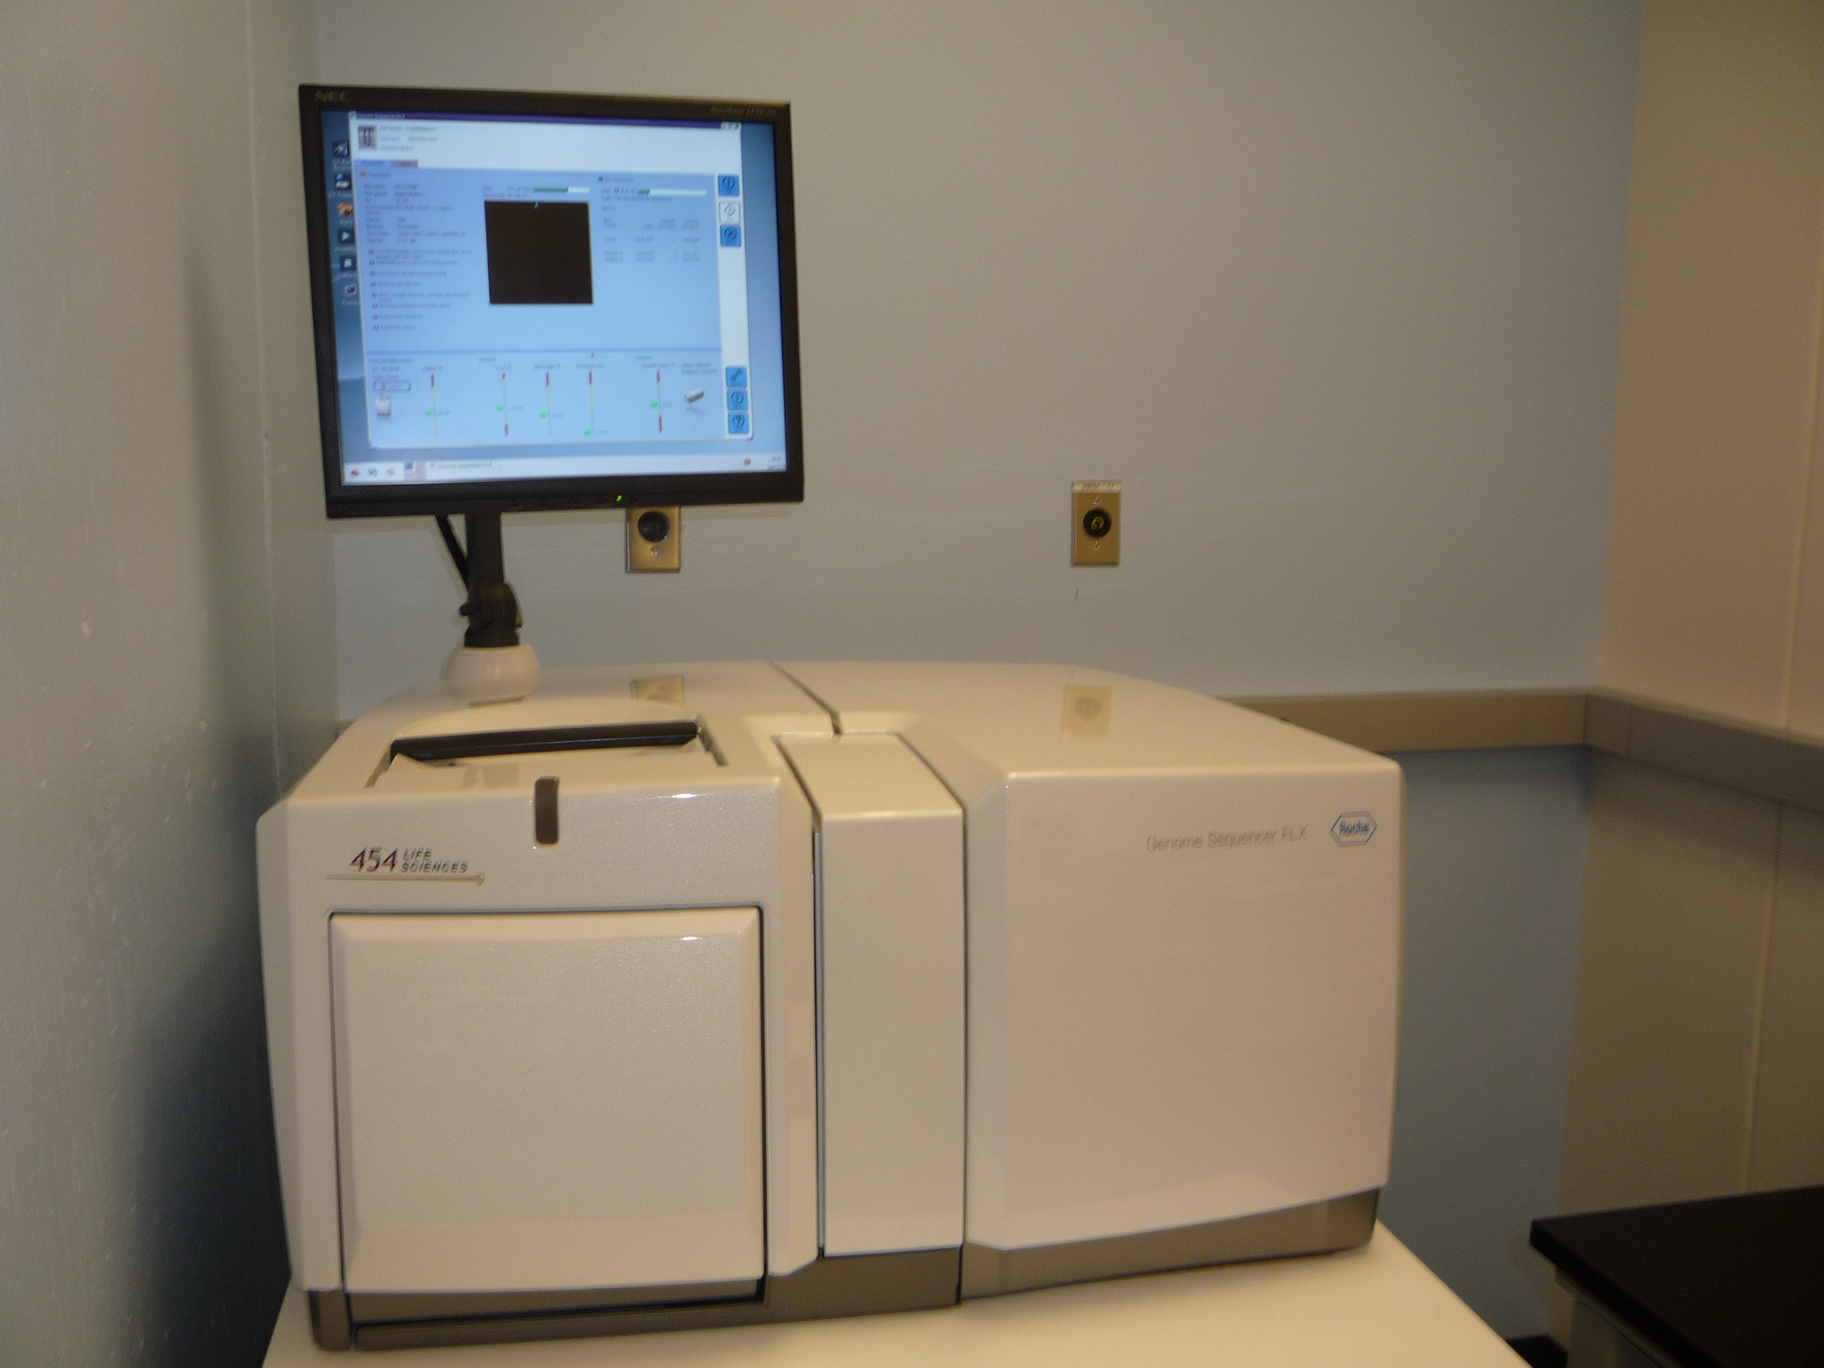
\includegraphics[width=1.0\textwidth]{454_Sequencer.jpg} \\
                454 Life Sciences Pyrosequencer \\
        \end{center}
    \end{minipage}
\end{frame}

\begin{frame}{Reads}
    \begin{itemize}
        \item A {\bf read} is a short sequence of base pairs that represents
        some DNA that was sequenced by the sequencing machine
        \item A read may come from any location in the genome, from either
        strand
        \item Reads from opposite strands always have opposite directions
            \begin{itemize}
                \item As a result, a sequence and its {\bf reverse-complement}
                (the corresponding sequence on the other strand, going
                backwards) are usually considered equivalent
            \end{itemize}
    \end{itemize}
        {\scriptsize
            {\tt \ \ }
            \hspace*{0.004cm}{\tt\color{red}$\leftarrow$TGAGCTTAAGGCTTATCTATCTTCAGACGACA$\leftarrow$ }\\
            {\tt \ \ }
            \hspace*{1.794cm}{\tt \color{red} $\leftarrow$TTATCTATCTTCAGACGACTATTATAGCGCGG$\leftarrow$}\\
            {\tt \ \ }
            {\tt $\leftarrow$TGAGCTTAAGGCTTATCTATCTTCAGACGACTATTATAGCGCGGCCAAGACTACGCGGAGCCCC$\leftarrow$} \\
            \vspace{-0.1cm}
            {\tt \ \ \ \ } {\tt |||||||||||||||||||||||||||||||||||||||||||||||||||||||||||||||| } \\
            \vspace{-0.1cm}
            {\tt \ \ }
            {\tt $\rightarrow$ACTCGAATTCCGAATAGATAGAAGTCTGCTGATAATATCGCGCCGGTTCTGATGCGCCTCGGGG$\rightarrow$} \\
            \vspace{-0.16cm}
            {\tt \ \ } \hspace*{3.585cm}{\tt \color{blue} $\rightarrow$TCTGCTGATAATATCGCGCCGGTTCTGATGCG$\rightarrow$}
            \vspace{0.5cm}
        }
        \\
        {Above: a very short genome and three reads that came from it}.
\end{frame}


\begin{frame}{Genome assembly}
    \begin{minipage}{0.63\textwidth}
        \begin{itemize}
            \item {\bf Genome assembly} is the process of reconstructing
                  a genome from a set of reads that came from it
            \item Genome assembly is performed by a complicated computer program
                called a genome {\bf assembler}
            \item Minimal input: a set of reads (35--5000 bp each), often in a
                simple plain-text format
            \item Minimal output: the reconstructed genome, or as close to it as
                possible (e.g. maximal length substrings)
        \end{itemize}
    \end{minipage}
    \begin{minipage}{0.35\textwidth}
        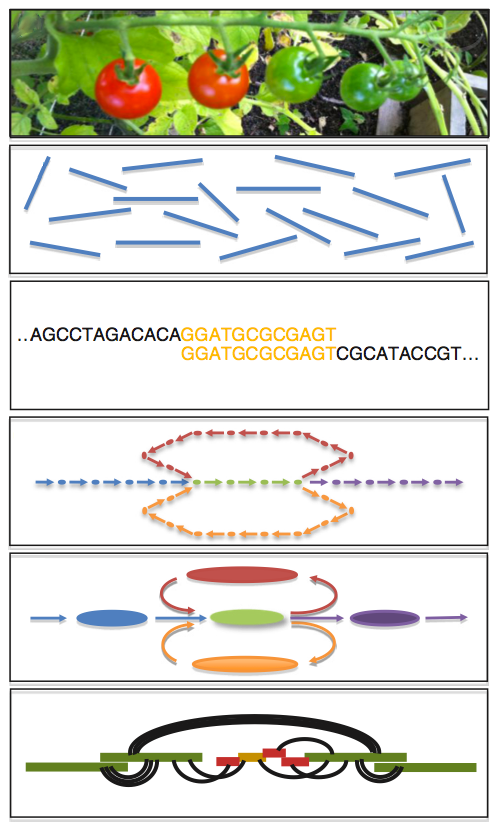
\includegraphics[width=0.97\textwidth]{AssemblyFlow.jpg}
    \end{minipage}
\end{frame}

\begin{frame}{Difficulties of genome assembly}
    \begin{itemize}
        \item The {\em Shortest Common Supersequence} (SCS) problem is
            NP-complete but is, in many ways, simpler than genome assembly
        \item Problems and issues not considered in this talk:
            \begin{itemize}
                \item Sequencing errors
                \item Heterozygosity
                \item Read duplication
                \item Sampling bias
                \item Contamination
                \item How to best make use of mate pair information
            \end{itemize}
        \item I {\em will} consider the double-stranded nature of DNA
    \end{itemize}
\end{frame}

\begin{frame}{An algorithm for genome assembly}
    \begin{itemize}
        \item Based on {\it The Fragment String Assembly Graph} (Myers 2005)
        \item Combines old and new ideas
        \item The overall algorithm:
        \begin{enumerate}
            \item Use overlaps to build a graph that models the assembly
            \item Simplify and analyze the graph
            \item Walk through the graph to reconstruct the original genome
        \end{enumerate}
        \item This talk won't cover the full algorithm; it only introduces the
              general graph-theoretical approach
    \end{itemize}
\end{frame}

\begin{frame}{Overlaps between reads}

    \begin{itemize}
    \item Two reads that overlap are likely to come from adjacent positions on
          the genome:
    \end{itemize}

    {\tt Read 1: \ \ \ \ \ \ \ \ \ $\rightarrow$
        ATATAT\textcolor{red}{GCTGGTTACTT} $\rightarrow$ } \\
    {\tt Read 2: \ \ \ \ \ \ \ \ \ \ \ \ \ \ \ $\rightarrow$
        \textcolor{red}{GCTGGTTACTT}TGATAGATA $\rightarrow$ } \\
    {\tt Possible genome: $\rightarrow$ ATATATGCTGGTTACTTTGATAGATA $\rightarrow$}

    \begin{itemize}
    \item Overlapping reads may be from different strands, in which case the
          overlapped regions are reverse-complement from each other:
    \end{itemize}

    {\tt Read 1: \ \ \ \ \ \ \ \ \ $\rightarrow$
        ATATAT\textcolor{red}{GCTGGTTACTT} $\rightarrow$ } \\
    {\tt Read 2: \ \ \ \ \ \ \ \ \ \ \ \ \ \ \ $\leftarrow$
        \textcolor{red}{CGACCAATGAA}ACTATCTAT $\leftarrow$ } \\
    {\tt Possible genome: $\rightarrow$ ATATATGCTGGTTACTTTGATAGATA $\rightarrow$}
\end{frame}

\begin{frame}{Three types of overlaps}
    \begin{enumerate}
        \item ``Normal'' overlap
            \begin{center}
                \vspace{-0.5cm}
                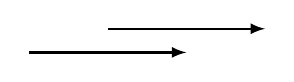
\begin{tikzpicture}[>=\ReadArrowType]
                    \draw[->,style=thick] (0,0) -- (2,0);
                    \draw[->,style=thick] (1.0,0.3) -- (3.0,0.3);
                \end{tikzpicture}

                \vspace{3mm}
                or (symmetrically)
                \vspace{3mm}

                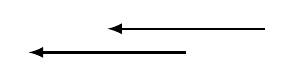
\begin{tikzpicture}[>=\ReadArrowType]
                    \draw[->,style=thick] (2,0) -- (0,0);
                    \draw[->,style=thick] (3.0,0.3) -- (1.0,0.3);
                \end{tikzpicture}
            \end{center}
        \vspace{0.5cm}
        \item ``Innie'' overlap
            \begin{center}
                \vspace{-0.5cm}
                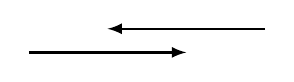
\begin{tikzpicture}[>=\ReadArrowType]
                    \draw[->,style=thick] (0,0) -- (2,0);
                    \draw[->,style=thick] (3,0.3) -- (1,0.3);
            \end{tikzpicture} \end{center}
        \vspace{0.5cm}
        \item ``Outie'' overlap
            \begin{center}
            \vspace{-0.5cm}
            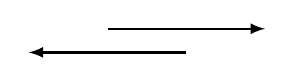
\begin{tikzpicture}[>=\ReadArrowType]
                    \draw[->,style=thick] (2,0) -- (0,0);
                    \draw[->,style=thick] (1.0,0.3) -- (3.0,0.3);
            \end{tikzpicture} \end{center}
    \end{enumerate}
\end{frame}

    %
    % Motivating example:                              
    %
    % 3 reads:
    %   f. ----------------->
    %   g. ----------------->
    %   h. ----------------->
    %
    % 3 overlaps:
    %   f. ------------------>
    %   g.        ---------------->
    %
    %   g. ------------------>
    %   h.       <------------------
    %
    %   f. ------------------->
    %   h.              <------------------
\begin{frame}{Towards a bidirected graph assembly model}
    %     <-----
    % GAATGCACAA
    % CTTACGTGTT
    % ----->
    %   ----->
    \vspace{-1.0cm}
    \begin{center}
        {\bf Motivating example}
    \end{center}
    \vspace{-0.5cm}
    \begin{minipage}{0.49\textwidth}
        3 reads:
        \begin{itemize}
            \item {\tt f. CTTACG$\rightarrow$}
            \item {\tt g. TACGTG$\rightarrow$}
            \item {\tt h. AACACG$\rightarrow$}
        \end{itemize}
        3 overlaps:
        \begin{itemize}
            \item {\tt f. CT\textcolor{red}{TACG}$\rightarrow$} \\
                {\tt g. \ \ \textcolor{red}{TACG}TG$\rightarrow$}

            \item {\tt g. TA\textcolor{red}{CGTG}$\rightarrow$} \\
                {\tt h. \hspace{0.023cm}$\leftarrow$\textcolor{red}{GCAC}AA}

            \item {\tt f. CTTA\textcolor{red}{CG}$\rightarrow$} \\
                {\tt h. \ \ \hspace{0.023cm}$\leftarrow$\textcolor{red}{GC}ACAA}
        \end{itemize}
    \end{minipage}
    \begin{minipage}{0.49\textwidth}
        \begin{itemize}
            \item Make a vertex for each read:
                \begin{center}
                    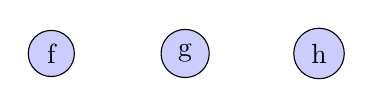
\begin{tikzpicture}[>=triangle 45]
                        \tikzstyle{every node} = [circle,fill=blue!20,draw=black];
                        \node (f) at (0, 0) {f};
                        \node (g) at (1.7, 0) {g};
                        \node (h) at (3.4, 0) {h};
                    \end{tikzpicture}
                \end{center}
            \item Make an edge for each overlap:
                \begin{center}
                    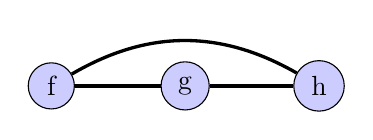
\begin{tikzpicture}[>=triangle 45]
                        \tikzstyle{every node} = [circle,fill=blue!20,draw=black];
                        \node (f) at (0, 0) {f};
                        \node (g) at (1.7, 0) {g};
                        \node (h) at (3.4, 0) {h};
                        \draw[style=very thick] (f) edge (g);
                        \draw[style=very thick] (g) edge (h);
                        \draw[style=very thick,bend left] (f) edge (h);
                    \end{tikzpicture}
                \end{center}
            \item But $...$ do undirected edges make sense here?
        \end{itemize}
    \end{minipage}
\end{frame}

\begin{frame}{Towards a bidirected graph assembly model}
    Possible {\bf undirected} and {\bf directed} graphs: \\
    \vspace{-0.5cm}
    \begin{center}
        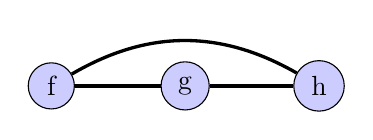
\begin{tikzpicture}[>=triangle 45]
            \tikzstyle{every node} = [circle,fill=blue!20,draw=black];
            \node (f) at (0, 0) {f};
            \node (g) at (1.7, 0) {g};
            \node (h) at (3.4, 0) {h};
            \draw[style=very thick] (f) edge (g);
            \draw[style=very thick] (g) edge (h);
            \draw[style=very thick,bend left] (f) edge (h);
        \end{tikzpicture}
        \hspace{1cm}
        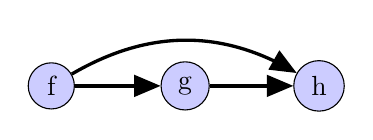
\begin{tikzpicture}[>=triangle 45]
            \tikzstyle{every node} = [circle,fill=blue!20,draw=black];
            \node (f) at (0, 0) {f};
            \node (g) at (1.7, 0) {g};
            \node (h) at (3.4, 0) {h};
            \draw[->,style=very thick] (f) edge (g);
            \draw[->,style=very thick] (g) edge (h);
            \draw[->,style=very thick,bend left] (f) edge (h);
        \end{tikzpicture}
    \end{center}
    \vspace{-0.2cm}
    Here's how we'd like to ``lay out'' and assemble the reads: \\
    \vspace{-0.2cm}
    \begin{center}
        \begin{tabular}{m{3.8cm}m{1.0cm}m{2.0cm}}
        {\tt f.\ CTTACG$\rightarrow$\ \ \ \ \ } \newline
        {\tt g.\ \ \ TACGTG$\rightarrow$\ \ \ } \newline
        {\tt h.\ \ \ \hspace{0.030cm}$\leftarrow$GCACAA\ \ \ }
        & $\Rightarrow$ & {\tt CTTACGTGTT} \\
        \end{tabular}
    \end{center}
    \vspace{-0.2cm}
    That is, we want to assemble $f \to g \to h$ OR $h \to g \to f$ OR $f \to h$ OR $h
    \to f$, BUT NOT something like $g \to h \to f$.
    Solution:  Use a {\bf bidirected} graph:
    \vspace{-0.2cm}
    \begin{center}
        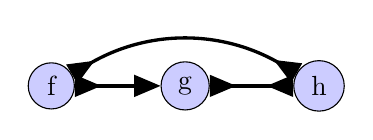
\begin{tikzpicture}[>=triangle 45]
            \tikzstyle{every node} = [circle,fill=blue!20,draw=black];
            \node (f) at (0, 0) {f};
            \node (g) at (1.7, 0) {g};
            \node (h) at (3.4, 0) {h};
            \draw[>->,style=very thick] (f) edge (g);
            \draw[>-<,style=very thick] (g) edge (h);
            \draw[>-<,style=very thick,bend left] (f) edge (h);
        \end{tikzpicture}
    \end{center}
\end{frame}

\begin{frame}{Bidirected Graphs}
    \begin{itemize}
        \item A {\bf bidirected graph} is a graph where a directed head is
        attached to both ends of each edge.

        \item There are 3 (or 4, ignoring symmetry) types of {\bf bidirected
        edges}.  They follow directly from the different types of overlaps.

        \begin{center}
            \begin{tabular}{p{1cm}cccc}
                {\footnotesize Overlap} &
                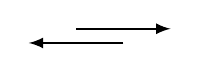
\begin{tikzpicture}[scale=0.6,>=\ReadArrowType]
                        \draw[->,style=thick] (2,0) -- (0,0);
                        \draw[->,style=thick] (1,0.3) -- (3,0.3);
                \end{tikzpicture}
                &
                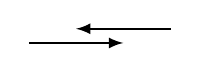
\begin{tikzpicture}[scale=0.6,>=\ReadArrowType]
                        \draw[->,style=thick] (0,0) -- (2,0);
                        \draw[->,style=thick] (3,0.3) -- (1,0.3);
                \end{tikzpicture}
                &
                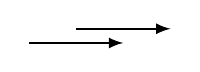
\begin{tikzpicture}[scale=0.6,>=\ReadArrowType]
                        \draw[->,style=thick] (0,0) -- (2,0);
                        \draw[->,style=thick] (1,0.3) -- (3,0.3);
                \end{tikzpicture}
                &
                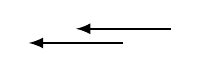
\begin{tikzpicture}[scale=0.6,>=\ReadArrowType]
                        \draw[->,style=thick] (2,0) -- (0,0);
                        \draw[->,style=thick] (3,0.3) -- (1,0.3);
                \end{tikzpicture}
                \\
                &$\downarrow$ & $\downarrow$& $\downarrow$& $\downarrow$ \\
                {\footnotesize Bidirected edge} &
                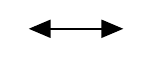
\begin{tikzpicture}[scale=0.6,>=triangle 45]
                        \draw[<->,style=thick] (0,0) -- (2,0);
                \end{tikzpicture}
                &
                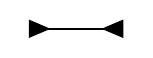
\begin{tikzpicture}[scale=0.6,>=triangle 45]
                        \draw[>-<,style=thick] (0,0) -- (2,0);
                \end{tikzpicture}
                &
                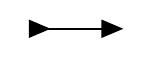
\begin{tikzpicture}[scale=0.6,>=triangle 45]
                        \draw[>->,style=thick] (0,0) -- (2,0);
                \end{tikzpicture}
                &
                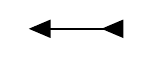
\begin{tikzpicture}[scale=0.6,>=triangle 45]
                        \draw[<-<,style=thick] (0,0) -- (2,0);
                \end{tikzpicture}
            \end{tabular}
        \end{center}
        %\item A {\bf walk in a bidirected graph} must pass through each vertex in a
            %consistent way.
        \item A {\bf walk in a bidirected graph} $G$ is a continuous sequence of
        edges in $G$ such that if any vertex $v$ is entered through a head
        inwards, it is exited through a head outwards (unless it is the end of the
        path), and vice versa.
        %\item Two vertices (reads) may have multiple {\bf bidirected edges}
        %between them if they overlap in different ways, but there can be at most
        %one bidirected edge {\em of the same type} between two vertices if we
        %always prefer the best overlap of a given type.
    \end{itemize}
\end{frame}


\begin{frame}{Walking through the bidirected string graph}
    \begin{itemize}
        \item A walk through a bidirected string graph constructed from
        reads and overlaps models a way in which the reads can be
        assembled together consistently.

        \item Each read may be used in forward or reverse-complement
        orientation, depending on the direction, relative to the walk,
        of the adjacent arrow heads when the corresponding vertex is
        passed through.
    \end{itemize}
    \begin{figure}[H]
        {\small
        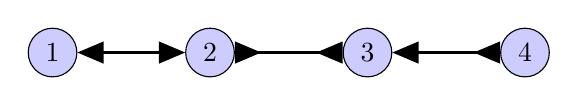
\begin{tikzpicture}[>=triangle 45]
            \tikzstyle{every node} = [circle,fill=blue!20,draw=black];
            \node (1) at (0.00, 0) {1};
            \node (2) at (2.0, 0) {2};
            \node (3) at (4.0, 0) {3};
            \node (4) at (6.0, 0) {4};
            \draw[<->,very thick] (1) edge (2);
            \draw[>-<,very thick] (2) edge (3);
            \draw[<-<,very thick] (3) edge (4);
        \end{tikzpicture} }

        \vspace{2.5mm}

        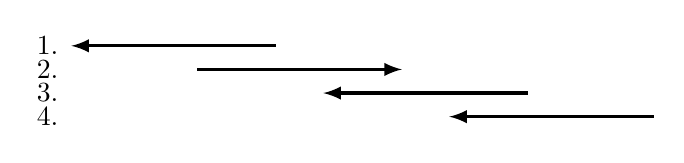
\begin{tikzpicture}[>=\ReadArrowType]
                \draw[<-,style=very thick] (0.0, 0.0) -- (2.6, 0.0);
                \draw[->,style=very thick] (1.6, -0.3) -- (4.2, -0.3);
                \draw[<-,style=very thick] (3.2, -0.6) -- (5.8, -0.6);
                \draw[<-,style=very thick] (4.8, -0.9) -- (7.4, -0.9);
                \draw (-0.3, 0.0) node {1.};
                \draw (-0.3, -0.3) node {2.};
                \draw (-0.3, -0.6) node {3.};
                \draw (-0.3, -0.9) node {4.};
        \end{tikzpicture}
        \caption{A bidirected graph and the implied assembly of the
        corresponding reads}
    \end{figure}
\end{frame}


%make -B SAMPLE_SIZE=450 out.reduced.mapped.bidigraph.pdf out.reduced.mapped.collapsed.bidigraph.pdf out.bidigraph.pdf GENOME=rep.fa COVERAGE=5

%make -B SAMPLE_SIZE=200 READ_LEN=50 MIN_OVERLAP_LEN=15 out.reduced.mapped.bidigraph.pdf out.reduced.mapped.collapsed.bidigraph.pdf out.bidigraph.pdf COVERAGE=3.0 SEED=5 USE_PIRS=false
\begin{frame}{Extremely small example}
    \begin{figure}[H]
        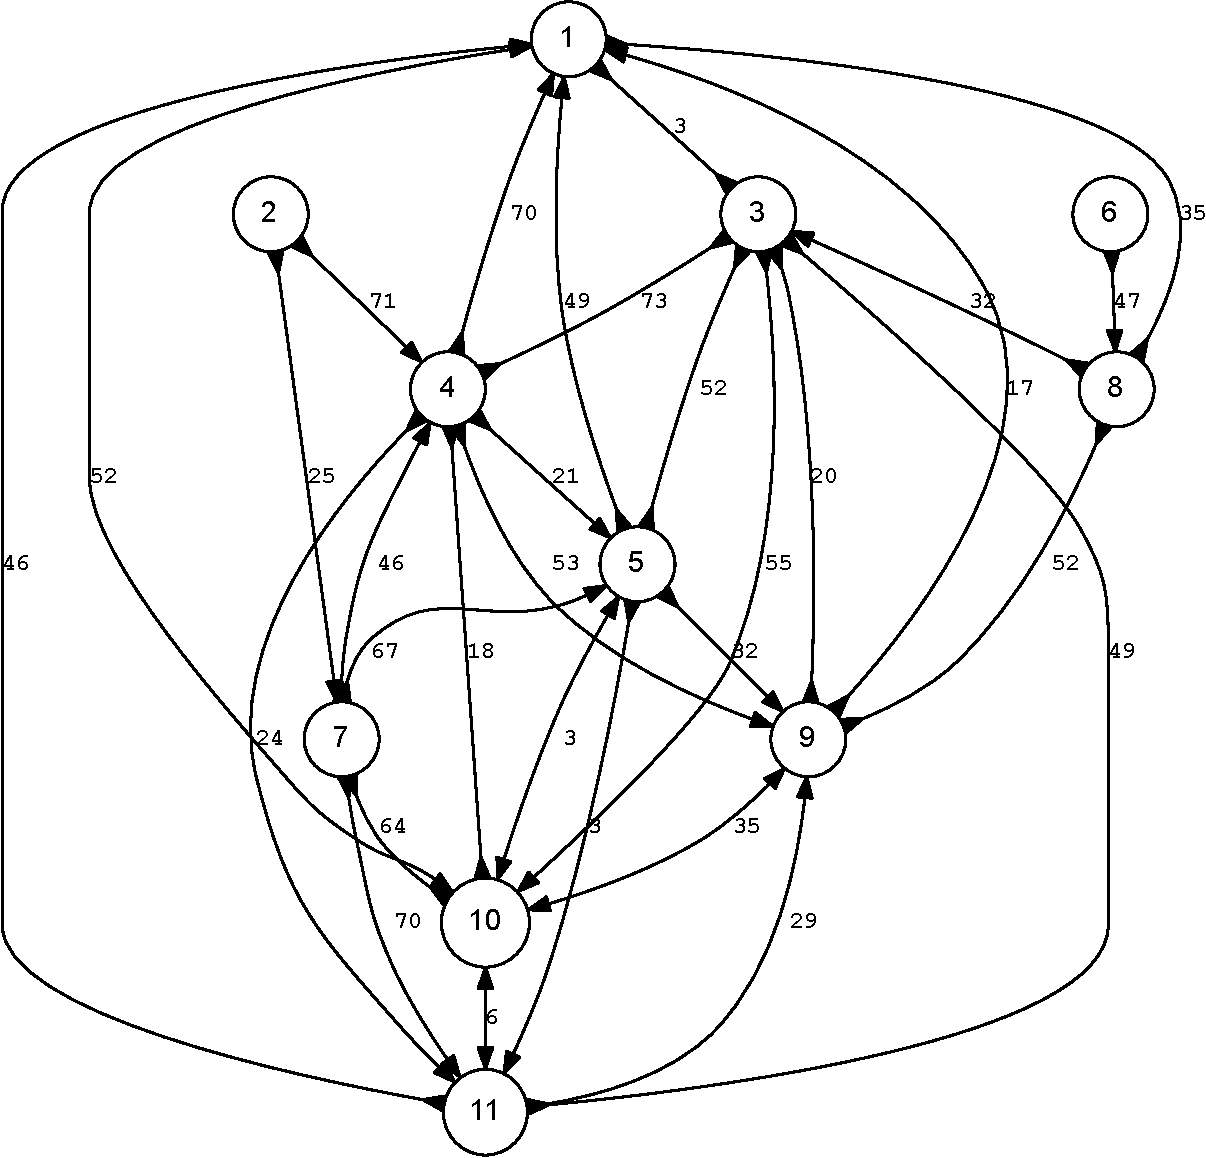
\includegraphics[scale=0.25]{example.bidigraph-crop.pdf}
        \caption{Bidirected string graph built from 100 bp reads sampled
        randomly at 5 $\times$ coverage from a 450 bp genome, using minimum 25
        bp overlaps.  Note: edges are labeled with the lengths of their DNA
        sequences (always the same each way in this example).}
    \end{figure}
\end{frame}

\begin{frame}{Extremely small example (cont.)}
    \begin{figure}[H]
        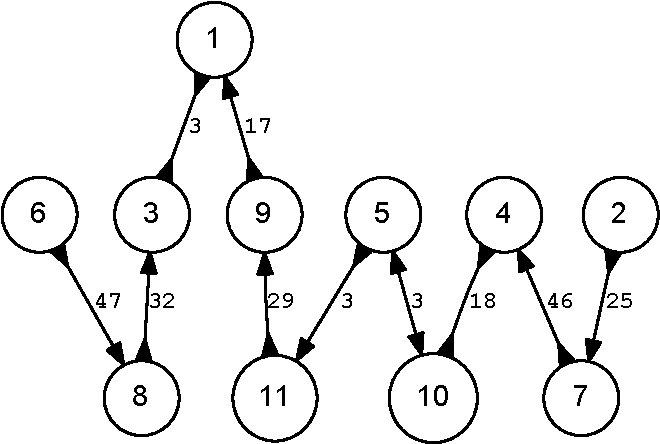
\includegraphics[scale=0.7]{example.reduced.mapped.bidigraph-crop.pdf}
        \caption{The bidirected string graph from the previous slide, after
        transitive reduction.}
    \end{figure}
\end{frame}

\begin{frame}{Extremely small example (cont.)}
    \begin{figure}[H]
        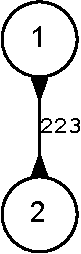
\includegraphics[scale=0.7]{example.reduced.mapped.collapsed.bidigraph-crop.pdf}
        \caption{The bidirected string graph from the previous slide, after
        collapsing unbranched paths.}
    \end{figure}
\end{frame}

\begin{frame}{Small example}
    \begin{itemize}
        \item Graph built from 1000bp reads sampled from {\it E. coli} genome
            (after transitive reduction \& collapsing unbranched paths)
    \end{itemize}
    \begin{center}
        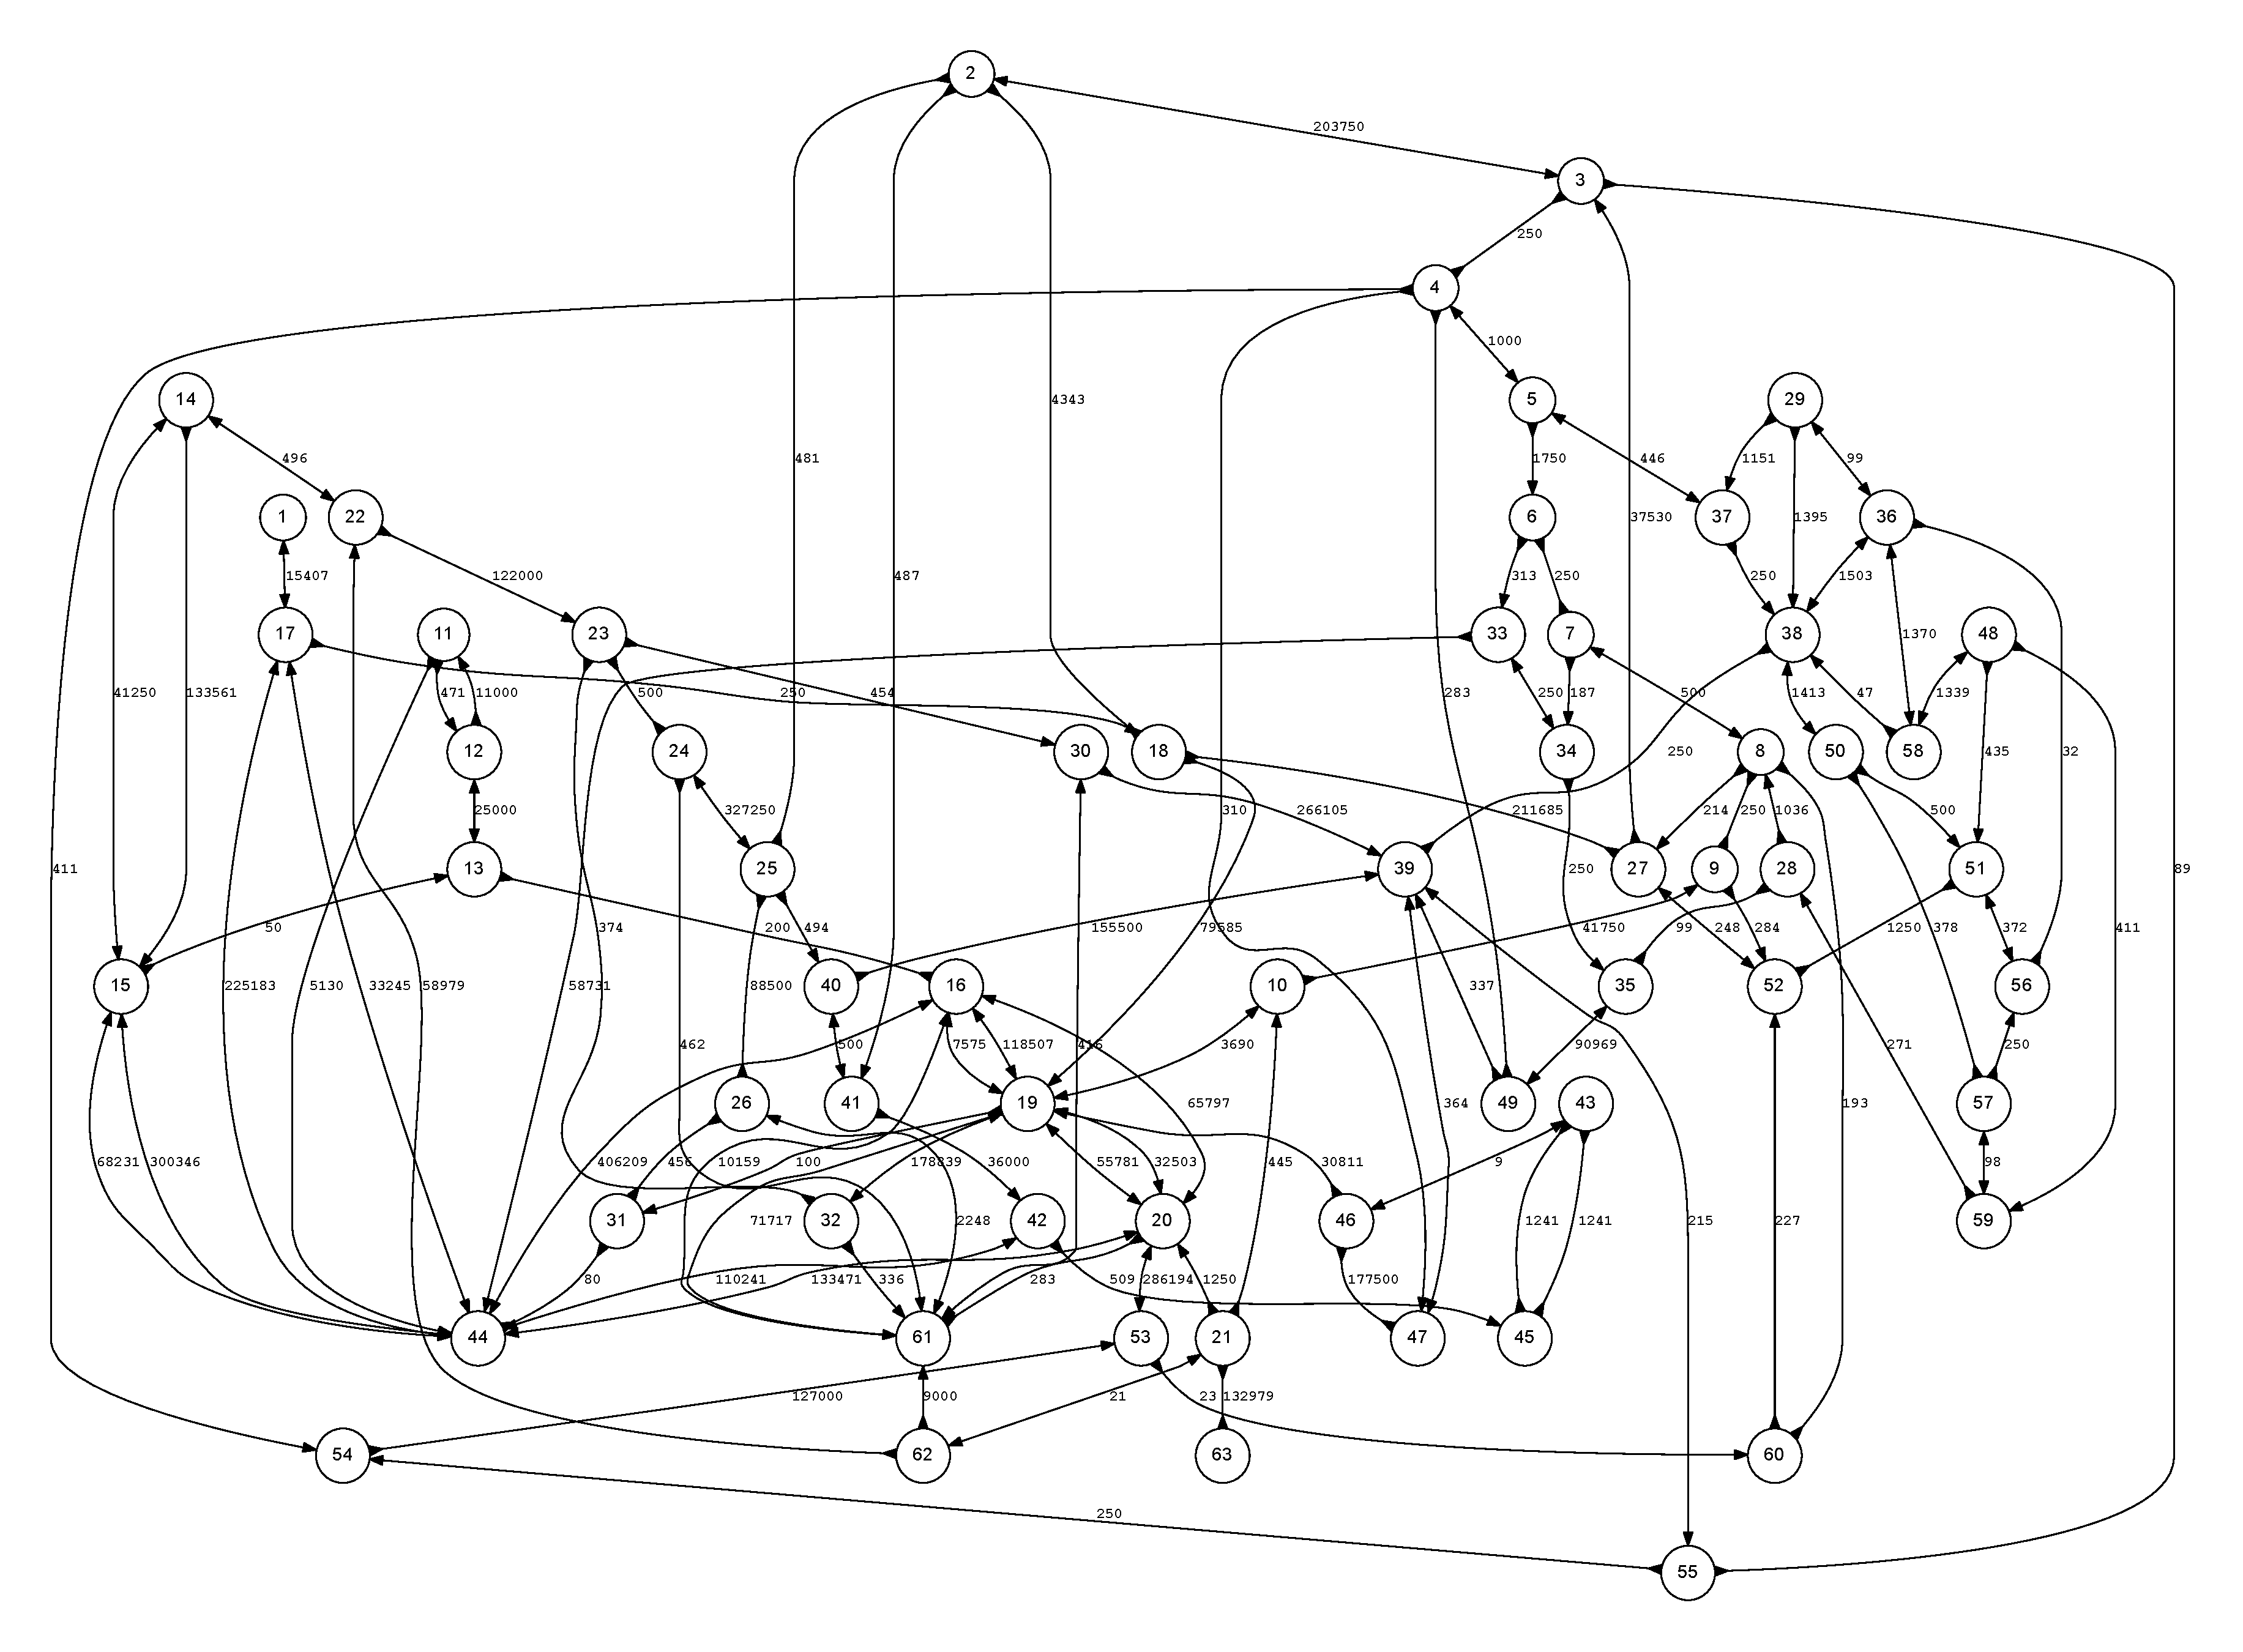
\includegraphics[width=0.8\textwidth]{E_coli.pdf}
    \end{center}
\end{frame}

\begin{frame}{Next steps}
    \begin{itemize}
        \item We need to determine the best way to walk through the graph to
            assemble the genome, but genomic repeats make the graph very
            complicated
        \item One approach:
            \begin{enumerate}
                \item Statistical analysis to determine approx. edge traversal counts
                \item Minimum-cost circulation {\bf on the bidirected graph} to
                      determine traversal counts
                \item Compute a generalized Eulerian cycle {\bf on the bidirected graph}
                      with dummy vertex added to allow discontinuities
                \item Read off the genome sequences from the generalized Eulerian cycle,
                      starting a new fragment whenever the dummy vertex is traversed
            \end{enumerate}
    \end{itemize}
\end{frame}

\begin{frame}{Acknowledgments}
    \begin{itemize}
        \item Talk advisor: Andrew Beveridge
        \item Project advisor: Stan Wagon
        \item {\em The fragment assembly string graph} (Eugene W. Myers, 2005)
        \item {\em Maximum likelihood genome assembly} (P. Medvedev  and M. Brudno, 2008)
        \item Also Michael Schatz at Cold Spring Harbor Laboratory, with whom
              I've worked on assembling the pineapple genome
    \end{itemize}
\end{frame}

\begin{frame}{Overlaps (formal definition)}
    Consider two reads, $f$ and $g$, and their reverse-complements $f'$ and $g'$.
    The reads $f$ and $g$ are said to {\bf exactly overlap} by some length
    $\LengthVar$ iff at least one of the following is true:
    \begin{itemize}
        \item The last $\LengthVar$ bp of $f$ exactly match the first
        $\LengthVar$ bp of $g$.
        \item The last $\LengthVar$ bp of $f$ exactly match the first
        $\LengthVar$ bp of $g'$.
        \item The last $\LengthVar$ bp of $f'$ exactly match the first
        $\LengthVar$ bp of $g$.
        \item The last $\LengthVar$ bp of $f'$ exactly match the first
        $\LengthVar$ bp of $g'$.
    \end{itemize}
    An overlap $o$ is fully described by the 7-tuple $(f, g, f_{begin}, f_{end},
    g_{begin}, g_{end}, rc)$.
    %there $f$ and $g$ are the reads of the overlap,
    %$f_{beg}$ and $g_{beg}$ and the starting position of the overlap on each
    %read, $len$ is the length of the overlap, and $rc$ indicates whether the
    %overlap is reverse-complement or not.
\end{frame}

\begin{frame}{Walks in a bidirected graph}
    \begin{itemize}
        \item A {\bf walk in a bidirected graph} $G$ is a continuous sequence of
        edges in $G$ such that if any vertex $v$ is entered through a head
        inwards, it is exited through a head outwards (unless it is the end of the
        path), and vice versa.
        \item A bidirected edge may be traversed in both directions
        (possibly even during the same walk).
        \item The reverse of a walk in a bidirected graph is also a
        valid walk.
        \item $1 \to 2 \to 3 \to 4$ and $4 \to 3 \to 2 \to 1$ are both valid
        walks in the bidirected graph below.  (Check circled pairs of
        heads.)
    \end{itemize}
        \begin{center} {\small
        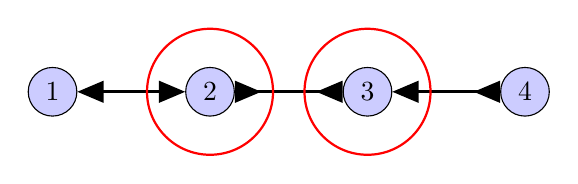
\begin{tikzpicture}[>=triangle 45]
            \tikzstyle{every node} = [circle,fill=blue!20,draw=black];
            \node (1) at (0.00, 0) {1};
            \node (2) at (2.00, 0) {2};
            \node (3) at (4.00, 0) {3};
            \node (4) at (6.00, 0) {4};
            \draw[<->,very thick] (1) edge (2);
            \draw[>-<,very thick] (2) edge (3);
            \draw[<-<,very thick] (3) edge (4);
            \draw[color=red,thick] (2.00, 0) circle (0.8);
            \draw[color=red,thick] (4.00, 0) circle (0.8);
        \end{tikzpicture} } \end{center}
\end{frame}

\begin{frame}{Walking through the bidirected string graph (cont.)}
    \begin{center}
        \vspace{-1cm}
        \begin{tabular}{p{3.6cm}c}
            \vspace{-1.5cm}
            {\small a.) A bidirected string graph fragment} &
            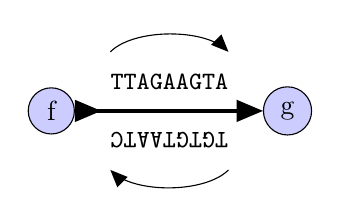
\begin{tikzpicture}[>=triangle 45,scale=1.5]
                \node[circle,fill=blue!20,draw=black] (f) at (0, 0) {f};
                \node[circle,fill=blue!20,draw=black] (g) at (2.0, 0) {g};
                \draw[>->,style=very thick] (f) edge (g);
                \draw (1.00, 0.1) node[anchor=south] {\small \tt TTAGAAGTA};
                \draw (1.00, -0.1) node[anchor=north] {
                        \rotatebox{180}{\small \tt
                        TGTGTAATC}};
                \draw[->] (0.5, 0.5) ..
                    controls (0.7, 0.7) and (1.3, 0.7) ..
                    (1.5, 0.5);
                \draw[->] (1.5, -0.5) ..
                    controls (1.3, -0.7) and (0.7, -0.7) ..
                    (0.5, -0.5);
            \end{tikzpicture}
            \\ \hline
            \vspace{-2.3cm}
            {\small b.) The corresponding overlap (labeled)
            %sequence
            %of overlapped region arbitrary as it is not known purely
            %from the graph fragment)
            } &
            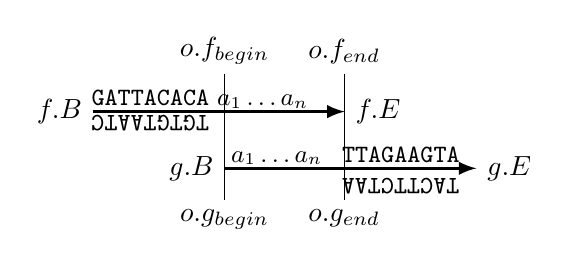
\begin{tikzpicture}[>=\ReadArrowType,scale=0.8]
                \draw[->,very thick] (0, 0) node[anchor=east] {$f.B$}
                        -> (4, 0) node[anchor=west] {$f.E$};
                \draw[->,very thick] (2.09, -0.9) node[anchor=east] {$g.B$}
                        -> (6.09, -0.9) node[anchor=west] {$g.E$};

                \draw (0, -0.1) node[anchor=south west]
                    {\hspace*{-1.4mm}{\small \tt
                        %GATTACACAGTGTAGTT
                        GATTACACA\hspace*{0.1cm}$a_1 \dots a_n$
                    }};

                \draw (0, 0.1) node[anchor=north west]
                    {\hspace*{-2.6mm}
                        \rotatebox{180}{{\small \tt TGTGTAATC}}};

                \draw (2.09, -1.0) node[anchor=south west]
                    {\hspace*{-1.4mm}{\small \tt
                        %GTGTAGTTTTAGAAGTA
                        \hspace*{0.1cm}$a_1 \dots a_n$\hspace*{0.25cm}TTAGAAGTA
                    }};

                \draw (2.09, -0.9) node[anchor=north west]
                    {\hspace*{12.48mm}
                        \rotatebox{180}{{\small \tt TACTTCTAA}}};

                \draw (2.09, -1.4) node[anchor=north] {$o.g_{begin}$}
                        -- (2.09, 0.6) node[anchor=south] {$o.f_{begin}$};
                \draw (3.99, -1.4) node[anchor=north] {$o.g_{end}$}
                        -- (3.99, 0.6) node[anchor=south] {$o.f_{end}$};
            \end{tikzpicture}
        \end{tabular}
    \end{center}
    \begin{tabular}{c|c}
        walk & interpretation \\ \hline
        $f \to g$ & $f.E \to g.E$ with sequence $g[o.g_{end} + 1 \dots ${\tt
        length}$(g)]$ \\
        $g \to f$ & $g.B \to f.B$ with sequence $f[o.g_{begin} - 1 \dots 0]$ \\
    \end{tabular}
    %\vspace{0.5cm}
    %\begin{itemize}
        %\item If we take {\bf each end} of {\bf each read} as a vertex, we can
        %make a directed graph equivalent to the bidirected graph.
    %\end{itemize}
\end{frame}

\begin{frame}{Transitive reduction}
	\begin{itemize}
		\item Very commonly, given three adjacent reads $f$, $g$, and $h$, $f$
		will overlap $h$ as well as $g$.  This is redundant because we can,
		equivalently, walk $f$ to $g$ to $h$ rather than directly walking from
		$f$ to $h$.

		\begin{center}
			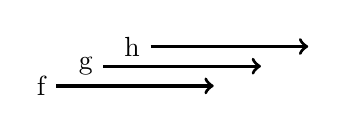
\begin{tikzpicture}
				\draw[->,style=very thick] (0,0) node[anchor=east] {f} -- (2,0);
				\draw[->,style=very thick] (0.6,0.25) node[anchor=east] {g} -- (2.6,0.25);
				\draw[->,style=very thick] (1.2,0.5) node[anchor=east] {h} -- (3.2,0.5);
			\end{tikzpicture}
			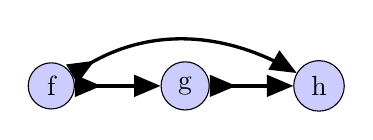
\begin{tikzpicture}[>=triangle 45]
				\tikzstyle{every node} = [circle,fill=blue!20,draw=black];
				\node (f) at (0, 0) {f};
				\node (g) at (1.7, 0) {g};
				\node (h) at (3.4, 0) {h};
				\draw[>->,style=very thick] (f) edge (g);
				\draw[>->,style=very thick] (g) edge (h);
				\draw[>->,style=very thick,bend left] (f) edge (h);
			\end{tikzpicture}
		\end{center}

		\item Walks visiting more vertices are preferred because they are
		supported by more reads and the overlaps tend to be longer.  So, we
		would like to throw away \BidirectedEdgeForward{$f$}{$h$} but keep
		\BidirectedEdgeForward{$f$}{$g$} and \BidirectedEdgeForward{$g$}{$h$}.

		\item To remove these redundant edges, {\bf transitive reduction} is
		performed on the bidirected string graph.
	\end{itemize}
\end{frame}

\begin{frame}{Arrival rate statistic (A-statistic)}
	\begin{itemize}
		\item The {\bf A-statistic} $A(e)$ of an edge $e$ in a
		bidirected string graph is:
	\end{itemize}
	\[ A(e) = \frac{n}{G} \Delta - \ln{2} \cdot {k} \]
	where $n$ is the total number of reads, $G$ is the estimated genome
	length, $\Delta$ is the length of the edge in bp, and $k$ is the number
	of reads that support that edge.
	\begin{itemize}
		\item The A-statistic is the logarithm of the probability that
		an edge represents unique sequence rather than duplicate
		sequence.
	\end{itemize}
\end{frame}

\begin{frame}{Implementation}
	\begin{minipage}{0.3\textwidth}
		\begin{itemize}
			\item A set of C++ programs that iteratively transform
			the data on-disk into the final assembly.
			\item Shaded programs are not yet implemented.
		\end{itemize}
	\end{minipage}
	\begin{minipage}{0.67\textwidth}
		\includegraphics[width=1.0\textwidth]{programs.pdf}
	\end{minipage}
\end{frame}

\end{document}
